% Capitolul 1: Date, randamente și indicatori
% Statistica piețelor financiare -- Program de licență, Academia de Studii Economice din București
% GENERAT de latex/build_chapter1.py -- modificați generatorul, nu acest fișier.

\newcommand{\coursename}{Statistica piețelor financiare}
\def\sfmlang{ro}
% Preambul comun SFM -- Statistica piețelor financiare / Statistics of Financial Markets (Beamer, 16:9)
% Același design ca MFM. Înainte de % Preambul comun SFM -- Statistica piețelor financiare / Statistics of Financial Markets (Beamer, 16:9)
% Același design ca MFM. Înainte de % Preambul comun SFM -- Statistica piețelor financiare / Statistics of Financial Markets (Beamer, 16:9)
% Același design ca MFM. Înainte de \input{../../latex/preamble} se definește
%   \newcommand{\coursename}{Statistics of Financial Markets}      (EN)
%   \newcommand{\coursename}{Statistica piețelor financiare}       (RO)  și  \def\sfmlang{ro}
% Fișierele .tex se află în EN/Courses, EN/Seminars, RO/Cursuri, RO/Seminarii (două niveluri sub rădăcină).
% Deck-urile sînt generate de latex/build_chapterN.py / build_seminarN.py (vezi latex/sfm_build.py).

\documentclass[9pt, aspectratio=169, t]{beamer}
\providecommand{\coursename}{Statistics of Financial Markets}

% Ensure content fits on slides
\setbeamersize{text margin left=8mm, text margin right=8mm}

%=============================================================================
% THEME AND STYLE CONFIGURATION
%=============================================================================
\usetheme{default}
% Using default theme for clean header/footer control

% Color Palette (matching Redispatch PDF)
\definecolor{MainBlue}{RGB}{26, 58, 110}
\definecolor{AccentBlue}{RGB}{26, 58, 110}
\definecolor{IDAred}{RGB}{205, 0, 0}
\definecolor{DarkGray}{RGB}{51, 51, 51}
\definecolor{MediumGray}{RGB}{128, 128, 128}
\definecolor{LightGray}{RGB}{248, 248, 248}
\definecolor{VeryLightGray}{RGB}{235, 235, 235}
\definecolor{KeynoteGray}{RGB}{218, 218, 218}
\definecolor{SectionGray}{RGB}{120, 120, 120}
\definecolor{FooterGray}{RGB}{100, 100, 100}
\definecolor{Crimson}{RGB}{220, 53, 69}
\definecolor{Forest}{RGB}{46, 125, 50}
\definecolor{Amber}{RGB}{181, 133, 63}
\definecolor{Orange}{RGB}{230, 126, 34}
\definecolor{Purple}{RGB}{142, 68, 173}

% Gradient background (exact Keynote 315° gradient: white to RGB 218,218,218)
\setbeamertemplate{background}{%
    \begin{tikzpicture}[remember picture, overlay]
        \shade[shading=axis, shading angle=315,
        top color=white, bottom color=KeynoteGray]
        (current page.south west) rectangle (current page.north east);
    \end{tikzpicture}%
}
% Fallback solid color for compatibility
\setbeamercolor{background canvas}{bg=}

\setbeamercolor{palette primary}{bg=MainBlue, fg=white}
\setbeamercolor{palette secondary}{bg=MainBlue!85, fg=white}
\setbeamercolor{palette tertiary}{bg=MainBlue!70, fg=white}
\setbeamercolor{structure}{fg=MainBlue}
\setbeamercolor{title}{fg=IDAred}
\setbeamercolor{frametitle}{fg=IDAred, bg=}
\setbeamercolor{block title}{bg=MainBlue, fg=white}
\setbeamercolor{block body}{bg=VeryLightGray, fg=DarkGray}
\setbeamercolor{block title alerted}{bg=Crimson, fg=white}
\setbeamercolor{block body alerted}{bg=Crimson!8, fg=DarkGray}
\setbeamercolor{block title example}{bg=Forest, fg=white}
\setbeamercolor{block body example}{bg=Forest!8, fg=DarkGray}
\setbeamercolor{item}{fg=MainBlue}

% Footer colors (override Madrid theme blue)
\setbeamercolor{author in head/foot}{fg=FooterGray, bg=}
\setbeamercolor{title in head/foot}{fg=FooterGray, bg=}
\setbeamercolor{date in head/foot}{fg=FooterGray, bg=}
\setbeamercolor{section in head/foot}{fg=FooterGray, bg=}
\setbeamercolor{subsection in head/foot}{fg=FooterGray, bg=}

% Bullet styles (apply everywhere including blocks)
\setbeamertemplate{itemize item}{\color{MainBlue}$\boxdot$}
\setbeamertemplate{itemize subitem}{\color{MainBlue}$\blacktriangleright$}
\setbeamertemplate{itemize subsubitem}{\color{MainBlue}\tiny$\bullet$}
\setbeamertemplate{itemize/enumerate body begin}{\normalsize}
\setbeamertemplate{itemize/enumerate subbody begin}{\normalsize}

% Item spacing - compact style
\setlength{\leftmargini}{10pt}       % Level 1: minimal indent
\setlength{\leftmarginii}{10pt}      % Level 2: minimal additional indent
% Compact list spacing (zero extra space before/after lists in blocks)
\makeatletter
\def\@listi{\leftmargin\leftmargini \topsep 0pt \parsep 0pt \itemsep 0pt}
\def\@listii{\leftmargin\leftmarginii \topsep 0pt \parsep 0pt \itemsep 0pt}
\makeatother

\setbeamertemplate{navigation symbols}{}

%=============================================================================
% CUSTOM HEADLINE
%=============================================================================
\setbeamertemplate{headline}{%
    \vskip10pt%
    \hbox to \paperwidth{%
        \hskip0.5cm%
        {\small\color{FooterGray}\renewcommand{\hyperlink}[2]{##2}\insertsectionhead}%
        \hfill%
        \textcolor{FooterGray}{\small\insertframenumber}%
        \hskip0.5cm%
    }%
    \vskip4pt%
    {\color{FooterGray}\hrule height 0.4pt}%
}

%=============================================================================
% CUSTOM FOOTER
%=============================================================================
\usepackage{fontawesome5}

\setbeamertemplate{footline}{%
    {\color{FooterGray}\hrule height 0.4pt}%
    \vskip4pt%
    \hbox to \paperwidth{%
        \hskip0.5cm%
        \textcolor{FooterGray}{\small\coursename}%
        \hfill%
        \raisebox{-0.1em}{%
            \begin{tikzpicture}[x=0.08em, y=0.08em, line width=0.4pt]
                \draw[FooterGray] (0,3) -- (1,4) -- (2,3.5) -- (3,5) -- (4,4) -- (5,6) -- (6,5.5) -- (7,4) -- (8,5) -- (9,7) -- (10,6) -- (11,5) -- (12,6.5) -- (13,8) -- (14,7) -- (15,6) -- (16,7.5) -- (17,9) -- (18,8) -- (19,7) -- (20,8.5) -- (21,10) -- (22,9) -- (23,8) -- (24,9.5);
            \end{tikzpicture}%
        }%
        \hskip0.5cm%
    }%
    \vskip6pt%
}

%=============================================================================
% PACKAGES
%=============================================================================
\usepackage[utf8]{inputenc}
\DeclareUnicodeCharacter{03B1}{\ensuremath{\alpha}}
\usepackage[T1]{fontenc}
\usepackage{amsmath, amssymb, amsthm}
\usepackage{mathtools}
\usepackage{bm}
\usepackage{tikz}
\usetikzlibrary{arrows.meta, positioning, shapes, calc, decorations.pathreplacing, shadings}
\usepackage{booktabs}
\usepackage{multirow}
\usepackage{array}
\usepackage{graphicx}
\usepackage{hyperref}
\usepackage{colortbl}
\usepackage{listings}
\lstset{language=Python, basicstyle=\ttfamily\scriptsize, keywordstyle=\color{MainBlue}\bfseries,
  commentstyle=\color{Forest}, stringstyle=\color{Crimson}, breaklines=true,
  frame=none, backgroundcolor=\color{VeryLightGray}, xleftmargin=2mm}
\hypersetup{colorlinks=true, linkcolor=MainBlue, urlcolor=MainBlue}
\graphicspath{{../../logos/}{../../charts/}{../../photos/}}
\usepackage{xcolor}
\hfuzz=2pt  % Suppress tiny overfull warnings (<2pt)
\vfuzz=2pt  % Suppress tiny vertical overfull warnings (<2pt)

%=============================================================================
% QUANTLET COMMANDS
%   \quantlet{<displayed name>}{<url>}       (generic, compatible with the older SFM decks)
%   \sfmquantlet{Ch_05}{SFM_ch5_garch}       -> https://github.com/danpele/SFM/tree/main/Quantlets/Ch_05/SFM_ch5_garch
%   \qlurl{<folder>} is defined per chapter by the generator (Quantlets/Ch_NN/<folder>)
%=============================================================================
\newcommand{\sfmrepo}{https://github.com/danpele/SFM}
\newcommand{\sfmqlbase}{https://github.com/danpele/SFM/tree/main/Quantlets}
\newcommand{\quantlet}[2]{%
    \hfill\href{#2}{%
        \raisebox{-0.15em}{
\includegraphics[height=0.7em]{ql_logo.png}}%
        \textcolor{MainBlue}{\tiny\ #1}%
    }%
}
\newcommand{\sfmquantlet}[2]{\quantlet{\detokenize{#2}}{\sfmqlbase/#1/#2}}

%=============================================================================
% NOTEBOOKS (Google Colab)
%   \colaburl{notebooks/EN/chapter5_seminar_notebook.ipynb} -> the Colab link of a file in the SFM repo
%   \nb: the chapter notebook (each seminar deck redefines it with \renewcommand)
%=============================================================================
\newcommand{\colaburl}[1]{https://colab.research.google.com/github/danpele/SFM/blob/main/#1}
\newcommand{\nb}{https://colab.research.google.com/github/danpele/SFM/tree/main/notebooks/EN}
\newcommand{\nbname}{notebooks/EN}

%=============================================================================
% SLIDE HELPERS (used by the generators; the same as in MFM)
%=============================================================================
% local font size for list bodies (the preamble forces \normalsize)
\newcommand{\itemsize}[1]{\setbeamertemplate{itemize/enumerate body begin}{#1}\setbeamertemplate{itemize/enumerate subbody begin}{#1}}
\newcommand{\intitle}[1]{{\hypersetup{urlcolor=white}#1}}   % white links inside coloured title bars
\newcommand{\imgcap}[1]{{\scriptsize #1}\\[0.5mm]}          % caption under a photo
\newcommand{\imgcredit}[2]{{\tiny\color{FooterGray}\href{#1}{#2}}}   % image credit: source URL, author/licence
\newcommand{\aiprompt}[1]{{\ttfamily\color{MainBlue}#1}}     % a prompt to an AI assistant

%=============================================================================
% SEMINARS: student version by default; the instructor wrapper *_solutions.tex sets \solutionstrue
%=============================================================================
\makeatletter\@ifundefined{ifsolutions}{\expandafter\newif\csname ifsolutions\endcsname}{}\makeatother
\newcommand{\solonly}[1]{\ifsolutions #1\fi}
\newcommand{\propsub}{\ifsolutions\else\framesubtitle{\ifdefined\sfmlang Rezolvarea se discută la seminar\else Solution discussed in class\fi}\fi}

%=============================================================================
% APPENDIX AND CHAPTER LINKS (latex/appendix_links.py writes the calls; it also re-declares these
% macros before \begin{document}, so the decks compile with or without this preamble block)
%=============================================================================
\providecommand{\sfmapplink}[3]{\hypertarget{#2}{}\hyperlink{#1}{\beamergotobutton{#3}}}
\providecommand{\sfmappback}[2]{\begin{tikzpicture}[remember picture,overlay]\node[anchor=south east] at ([xshift=-3mm,yshift=7mm]current page.south east){\hyperlink{#1}{\beamerreturnbutton{#2}}};\end{tikzpicture}}
\providecommand{\sfmchlink}[2]{\href{#1}{#2}}
\providecommand{\sfmchlinkt}[2]{\href{#1}{\usebeamercolor[fg]{frametitle}#2}}

%=============================================================================
% QUANTINAR COMMAND: link către un curs Quantinar (subiecte avansate)
%=============================================================================
\newcommand{\quantinar}[2]{%
    \href{#2}{%
        \raisebox{-0.15em}{
\includegraphics[height=0.8em]{qr_logo.png}}%
        \textcolor{MainBlue}{\scriptsize\ #1}%
    }%
}

%=============================================================================
% CUSTOM TITLE PAGE
%=============================================================================
\defbeamertemplate*{title page}{hybrid}[1][]
{
    \vspace{0.2cm}
    % Logos row - top header (with clickable links)
    \begin{center}
        \href{https://www.ase.ro}{
\includegraphics[height=1.0cm]{ase_logo.png}}\hspace{0.3cm}%
        \href{https://theida.net}{
\includegraphics[height=1.0cm]{ida_logo.png}}\hspace{0.3cm}%
        \href{https://blockchain-research-center.com}{
\includegraphics[height=1.0cm]{brc_logo.png}}\hspace{0.3cm}%
        \href{https://www.ai4efin.ase.ro}{
\includegraphics[height=1.0cm]{ai4efin_logo.png}}\hspace{0.3cm}%
        \href{https://ipe.ro/new}{
\includegraphics[height=1.0cm]{acad_logo.png}}\hspace{0.3cm}%
        \href{https://www.digital-finance-msca.com}{
\includegraphics[height=1.0cm]{msca_logo.png}}%
    \end{center}

    \vspace{0.6cm}

    % Main title with Q logos on sides (with clickable links)
    \begin{center}
        \begin{minipage}{0.1\textwidth}
            \centering
            \href{https://quantlet.com}{
\includegraphics[height=1.1cm]{ql_logo.png}}
        \end{minipage}%
        \begin{minipage}{0.78\textwidth}
            \centering
            {\LARGE\bfseries\usebeamercolor[fg]{title}\inserttitle}

            \vspace{0.3cm}

            {\usebeamerfont{subtitle}\usebeamercolor[fg]{title}\insertsubtitle}
        \end{minipage}%
        \begin{minipage}{0.1\textwidth}
            \centering
            \href{https://quantinar.com}{
\includegraphics[height=1.1cm]{qr_logo.png}}
        \end{minipage}
    \end{center}

    \vspace{0.6cm}

    % Authors (left aligned)
    \hspace{0.5cm}{\usebeamerfont{author}\insertauthor}

    \vspace{0.3cm}

    % Institute/Affiliations (left aligned)
    \hspace{0.5cm}\begin{minipage}[t]{0.9\textwidth}
        \raggedright\small\insertinstitute
    \end{minipage}
}

%=============================================================================
% THEOREM ENVIRONMENTS
%=============================================================================
\theoremstyle{definition}
\setbeamertemplate{theorems}[numbered]
\ifdefined\sfmlang
\newtheorem{defn}{Definiție}
\newtheorem{thm}{Teoremă}
\newtheorem{prop}{Propoziție}
\newtheorem{rmk}{Observație}
\else
\newtheorem{defn}{Definition}
\newtheorem{thm}{Theorem}
\newtheorem{prop}{Proposition}
\newtheorem{rmk}{Remark}
\fi

%=============================================================================
% CENTRED MINIPAGE (no extra vertical space)
%=============================================================================
\newenvironment{cminipage}[1]{%
    \par\noindent\hfill\begin{minipage}{#1}\ignorespaces
}{%
    \end{minipage}\hfill\null\par
}

%=============================================================================
% CUSTOM COMMANDS
%=============================================================================
\newcommand{\E}{\mathbb{E}}
\newcommand{\Var}{\text{Var}}
\newcommand{\Cov}{\text{Cov}}
\newcommand{\Corr}{\text{Corr}}
\newcommand{\R}{\mathbb{R}}
\newcommand{\N}{\mathbb{N}}
\newcommand{\Z}{\mathbb{Z}}
\newcommand{\B}{\mathbf{B}}
\newcommand{\imark}{\textcolor{MainBlue}{\textbullet}}
\newcommand{\RMSE}{\text{RMSE}}
\newcommand{\MAE}{\text{MAE}}
\newcommand{\MAPE}{\text{MAPE}}

 se definește
%   \newcommand{\coursename}{Statistics of Financial Markets}      (EN)
%   \newcommand{\coursename}{Statistica piețelor financiare}       (RO)  și  \def\sfmlang{ro}
% Fișierele .tex se află în EN/Courses, EN/Seminars, RO/Cursuri, RO/Seminarii (două niveluri sub rădăcină).
% Deck-urile sînt generate de latex/build_chapterN.py / build_seminarN.py (vezi latex/sfm_build.py).

\documentclass[9pt, aspectratio=169, t]{beamer}
\providecommand{\coursename}{Statistics of Financial Markets}

% Ensure content fits on slides
\setbeamersize{text margin left=8mm, text margin right=8mm}

%=============================================================================
% THEME AND STYLE CONFIGURATION
%=============================================================================
\usetheme{default}
% Using default theme for clean header/footer control

% Color Palette (matching Redispatch PDF)
\definecolor{MainBlue}{RGB}{26, 58, 110}
\definecolor{AccentBlue}{RGB}{26, 58, 110}
\definecolor{IDAred}{RGB}{205, 0, 0}
\definecolor{DarkGray}{RGB}{51, 51, 51}
\definecolor{MediumGray}{RGB}{128, 128, 128}
\definecolor{LightGray}{RGB}{248, 248, 248}
\definecolor{VeryLightGray}{RGB}{235, 235, 235}
\definecolor{KeynoteGray}{RGB}{218, 218, 218}
\definecolor{SectionGray}{RGB}{120, 120, 120}
\definecolor{FooterGray}{RGB}{100, 100, 100}
\definecolor{Crimson}{RGB}{220, 53, 69}
\definecolor{Forest}{RGB}{46, 125, 50}
\definecolor{Amber}{RGB}{181, 133, 63}
\definecolor{Orange}{RGB}{230, 126, 34}
\definecolor{Purple}{RGB}{142, 68, 173}

% Gradient background (exact Keynote 315° gradient: white to RGB 218,218,218)
\setbeamertemplate{background}{%
    \begin{tikzpicture}[remember picture, overlay]
        \shade[shading=axis, shading angle=315,
        top color=white, bottom color=KeynoteGray]
        (current page.south west) rectangle (current page.north east);
    \end{tikzpicture}%
}
% Fallback solid color for compatibility
\setbeamercolor{background canvas}{bg=}

\setbeamercolor{palette primary}{bg=MainBlue, fg=white}
\setbeamercolor{palette secondary}{bg=MainBlue!85, fg=white}
\setbeamercolor{palette tertiary}{bg=MainBlue!70, fg=white}
\setbeamercolor{structure}{fg=MainBlue}
\setbeamercolor{title}{fg=IDAred}
\setbeamercolor{frametitle}{fg=IDAred, bg=}
\setbeamercolor{block title}{bg=MainBlue, fg=white}
\setbeamercolor{block body}{bg=VeryLightGray, fg=DarkGray}
\setbeamercolor{block title alerted}{bg=Crimson, fg=white}
\setbeamercolor{block body alerted}{bg=Crimson!8, fg=DarkGray}
\setbeamercolor{block title example}{bg=Forest, fg=white}
\setbeamercolor{block body example}{bg=Forest!8, fg=DarkGray}
\setbeamercolor{item}{fg=MainBlue}

% Footer colors (override Madrid theme blue)
\setbeamercolor{author in head/foot}{fg=FooterGray, bg=}
\setbeamercolor{title in head/foot}{fg=FooterGray, bg=}
\setbeamercolor{date in head/foot}{fg=FooterGray, bg=}
\setbeamercolor{section in head/foot}{fg=FooterGray, bg=}
\setbeamercolor{subsection in head/foot}{fg=FooterGray, bg=}

% Bullet styles (apply everywhere including blocks)
\setbeamertemplate{itemize item}{\color{MainBlue}$\boxdot$}
\setbeamertemplate{itemize subitem}{\color{MainBlue}$\blacktriangleright$}
\setbeamertemplate{itemize subsubitem}{\color{MainBlue}\tiny$\bullet$}
\setbeamertemplate{itemize/enumerate body begin}{\normalsize}
\setbeamertemplate{itemize/enumerate subbody begin}{\normalsize}

% Item spacing - compact style
\setlength{\leftmargini}{10pt}       % Level 1: minimal indent
\setlength{\leftmarginii}{10pt}      % Level 2: minimal additional indent
% Compact list spacing (zero extra space before/after lists in blocks)
\makeatletter
\def\@listi{\leftmargin\leftmargini \topsep 0pt \parsep 0pt \itemsep 0pt}
\def\@listii{\leftmargin\leftmarginii \topsep 0pt \parsep 0pt \itemsep 0pt}
\makeatother

\setbeamertemplate{navigation symbols}{}

%=============================================================================
% CUSTOM HEADLINE
%=============================================================================
\setbeamertemplate{headline}{%
    \vskip10pt%
    \hbox to \paperwidth{%
        \hskip0.5cm%
        {\small\color{FooterGray}\renewcommand{\hyperlink}[2]{##2}\insertsectionhead}%
        \hfill%
        \textcolor{FooterGray}{\small\insertframenumber}%
        \hskip0.5cm%
    }%
    \vskip4pt%
    {\color{FooterGray}\hrule height 0.4pt}%
}

%=============================================================================
% CUSTOM FOOTER
%=============================================================================
\usepackage{fontawesome5}

\setbeamertemplate{footline}{%
    {\color{FooterGray}\hrule height 0.4pt}%
    \vskip4pt%
    \hbox to \paperwidth{%
        \hskip0.5cm%
        \textcolor{FooterGray}{\small\coursename}%
        \hfill%
        \raisebox{-0.1em}{%
            \begin{tikzpicture}[x=0.08em, y=0.08em, line width=0.4pt]
                \draw[FooterGray] (0,3) -- (1,4) -- (2,3.5) -- (3,5) -- (4,4) -- (5,6) -- (6,5.5) -- (7,4) -- (8,5) -- (9,7) -- (10,6) -- (11,5) -- (12,6.5) -- (13,8) -- (14,7) -- (15,6) -- (16,7.5) -- (17,9) -- (18,8) -- (19,7) -- (20,8.5) -- (21,10) -- (22,9) -- (23,8) -- (24,9.5);
            \end{tikzpicture}%
        }%
        \hskip0.5cm%
    }%
    \vskip6pt%
}

%=============================================================================
% PACKAGES
%=============================================================================
\usepackage[utf8]{inputenc}
\DeclareUnicodeCharacter{03B1}{\ensuremath{\alpha}}
\usepackage[T1]{fontenc}
\usepackage{amsmath, amssymb, amsthm}
\usepackage{mathtools}
\usepackage{bm}
\usepackage{tikz}
\usetikzlibrary{arrows.meta, positioning, shapes, calc, decorations.pathreplacing, shadings}
\usepackage{booktabs}
\usepackage{multirow}
\usepackage{array}
\usepackage{graphicx}
\usepackage{hyperref}
\usepackage{colortbl}
\usepackage{listings}
\lstset{language=Python, basicstyle=\ttfamily\scriptsize, keywordstyle=\color{MainBlue}\bfseries,
  commentstyle=\color{Forest}, stringstyle=\color{Crimson}, breaklines=true,
  frame=none, backgroundcolor=\color{VeryLightGray}, xleftmargin=2mm}
\hypersetup{colorlinks=true, linkcolor=MainBlue, urlcolor=MainBlue}
\graphicspath{{../../logos/}{../../charts/}{../../photos/}}
\usepackage{xcolor}
\hfuzz=2pt  % Suppress tiny overfull warnings (<2pt)
\vfuzz=2pt  % Suppress tiny vertical overfull warnings (<2pt)

%=============================================================================
% QUANTLET COMMANDS
%   \quantlet{<displayed name>}{<url>}       (generic, compatible with the older SFM decks)
%   \sfmquantlet{Ch_05}{SFM_ch5_garch}       -> https://github.com/danpele/SFM/tree/main/Quantlets/Ch_05/SFM_ch5_garch
%   \qlurl{<folder>} is defined per chapter by the generator (Quantlets/Ch_NN/<folder>)
%=============================================================================
\newcommand{\sfmrepo}{https://github.com/danpele/SFM}
\newcommand{\sfmqlbase}{https://github.com/danpele/SFM/tree/main/Quantlets}
\newcommand{\quantlet}[2]{%
    \hfill\href{#2}{%
        \raisebox{-0.15em}{
\includegraphics[height=0.7em]{ql_logo.png}}%
        \textcolor{MainBlue}{\tiny\ #1}%
    }%
}
\newcommand{\sfmquantlet}[2]{\quantlet{\detokenize{#2}}{\sfmqlbase/#1/#2}}

%=============================================================================
% NOTEBOOKS (Google Colab)
%   \colaburl{notebooks/EN/chapter5_seminar_notebook.ipynb} -> the Colab link of a file in the SFM repo
%   \nb: the chapter notebook (each seminar deck redefines it with \renewcommand)
%=============================================================================
\newcommand{\colaburl}[1]{https://colab.research.google.com/github/danpele/SFM/blob/main/#1}
\newcommand{\nb}{https://colab.research.google.com/github/danpele/SFM/tree/main/notebooks/EN}
\newcommand{\nbname}{notebooks/EN}

%=============================================================================
% SLIDE HELPERS (used by the generators; the same as in MFM)
%=============================================================================
% local font size for list bodies (the preamble forces \normalsize)
\newcommand{\itemsize}[1]{\setbeamertemplate{itemize/enumerate body begin}{#1}\setbeamertemplate{itemize/enumerate subbody begin}{#1}}
\newcommand{\intitle}[1]{{\hypersetup{urlcolor=white}#1}}   % white links inside coloured title bars
\newcommand{\imgcap}[1]{{\scriptsize #1}\\[0.5mm]}          % caption under a photo
\newcommand{\imgcredit}[2]{{\tiny\color{FooterGray}\href{#1}{#2}}}   % image credit: source URL, author/licence
\newcommand{\aiprompt}[1]{{\ttfamily\color{MainBlue}#1}}     % a prompt to an AI assistant

%=============================================================================
% SEMINARS: student version by default; the instructor wrapper *_solutions.tex sets \solutionstrue
%=============================================================================
\makeatletter\@ifundefined{ifsolutions}{\expandafter\newif\csname ifsolutions\endcsname}{}\makeatother
\newcommand{\solonly}[1]{\ifsolutions #1\fi}
\newcommand{\propsub}{\ifsolutions\else\framesubtitle{\ifdefined\sfmlang Rezolvarea se discută la seminar\else Solution discussed in class\fi}\fi}

%=============================================================================
% APPENDIX AND CHAPTER LINKS (latex/appendix_links.py writes the calls; it also re-declares these
% macros before \begin{document}, so the decks compile with or without this preamble block)
%=============================================================================
\providecommand{\sfmapplink}[3]{\hypertarget{#2}{}\hyperlink{#1}{\beamergotobutton{#3}}}
\providecommand{\sfmappback}[2]{\begin{tikzpicture}[remember picture,overlay]\node[anchor=south east] at ([xshift=-3mm,yshift=7mm]current page.south east){\hyperlink{#1}{\beamerreturnbutton{#2}}};\end{tikzpicture}}
\providecommand{\sfmchlink}[2]{\href{#1}{#2}}
\providecommand{\sfmchlinkt}[2]{\href{#1}{\usebeamercolor[fg]{frametitle}#2}}

%=============================================================================
% QUANTINAR COMMAND: link către un curs Quantinar (subiecte avansate)
%=============================================================================
\newcommand{\quantinar}[2]{%
    \href{#2}{%
        \raisebox{-0.15em}{
\includegraphics[height=0.8em]{qr_logo.png}}%
        \textcolor{MainBlue}{\scriptsize\ #1}%
    }%
}

%=============================================================================
% CUSTOM TITLE PAGE
%=============================================================================
\defbeamertemplate*{title page}{hybrid}[1][]
{
    \vspace{0.2cm}
    % Logos row - top header (with clickable links)
    \begin{center}
        \href{https://www.ase.ro}{
\includegraphics[height=1.0cm]{ase_logo.png}}\hspace{0.3cm}%
        \href{https://theida.net}{
\includegraphics[height=1.0cm]{ida_logo.png}}\hspace{0.3cm}%
        \href{https://blockchain-research-center.com}{
\includegraphics[height=1.0cm]{brc_logo.png}}\hspace{0.3cm}%
        \href{https://www.ai4efin.ase.ro}{
\includegraphics[height=1.0cm]{ai4efin_logo.png}}\hspace{0.3cm}%
        \href{https://ipe.ro/new}{
\includegraphics[height=1.0cm]{acad_logo.png}}\hspace{0.3cm}%
        \href{https://www.digital-finance-msca.com}{
\includegraphics[height=1.0cm]{msca_logo.png}}%
    \end{center}

    \vspace{0.6cm}

    % Main title with Q logos on sides (with clickable links)
    \begin{center}
        \begin{minipage}{0.1\textwidth}
            \centering
            \href{https://quantlet.com}{
\includegraphics[height=1.1cm]{ql_logo.png}}
        \end{minipage}%
        \begin{minipage}{0.78\textwidth}
            \centering
            {\LARGE\bfseries\usebeamercolor[fg]{title}\inserttitle}

            \vspace{0.3cm}

            {\usebeamerfont{subtitle}\usebeamercolor[fg]{title}\insertsubtitle}
        \end{minipage}%
        \begin{minipage}{0.1\textwidth}
            \centering
            \href{https://quantinar.com}{
\includegraphics[height=1.1cm]{qr_logo.png}}
        \end{minipage}
    \end{center}

    \vspace{0.6cm}

    % Authors (left aligned)
    \hspace{0.5cm}{\usebeamerfont{author}\insertauthor}

    \vspace{0.3cm}

    % Institute/Affiliations (left aligned)
    \hspace{0.5cm}\begin{minipage}[t]{0.9\textwidth}
        \raggedright\small\insertinstitute
    \end{minipage}
}

%=============================================================================
% THEOREM ENVIRONMENTS
%=============================================================================
\theoremstyle{definition}
\setbeamertemplate{theorems}[numbered]
\ifdefined\sfmlang
\newtheorem{defn}{Definiție}
\newtheorem{thm}{Teoremă}
\newtheorem{prop}{Propoziție}
\newtheorem{rmk}{Observație}
\else
\newtheorem{defn}{Definition}
\newtheorem{thm}{Theorem}
\newtheorem{prop}{Proposition}
\newtheorem{rmk}{Remark}
\fi

%=============================================================================
% CENTRED MINIPAGE (no extra vertical space)
%=============================================================================
\newenvironment{cminipage}[1]{%
    \par\noindent\hfill\begin{minipage}{#1}\ignorespaces
}{%
    \end{minipage}\hfill\null\par
}

%=============================================================================
% CUSTOM COMMANDS
%=============================================================================
\newcommand{\E}{\mathbb{E}}
\newcommand{\Var}{\text{Var}}
\newcommand{\Cov}{\text{Cov}}
\newcommand{\Corr}{\text{Corr}}
\newcommand{\R}{\mathbb{R}}
\newcommand{\N}{\mathbb{N}}
\newcommand{\Z}{\mathbb{Z}}
\newcommand{\B}{\mathbf{B}}
\newcommand{\imark}{\textcolor{MainBlue}{\textbullet}}
\newcommand{\RMSE}{\text{RMSE}}
\newcommand{\MAE}{\text{MAE}}
\newcommand{\MAPE}{\text{MAPE}}

 se definește
%   \newcommand{\coursename}{Statistics of Financial Markets}      (EN)
%   \newcommand{\coursename}{Statistica piețelor financiare}       (RO)  și  \def\sfmlang{ro}
% Fișierele .tex se află în EN/Courses, EN/Seminars, RO/Cursuri, RO/Seminarii (două niveluri sub rădăcină).
% Deck-urile sînt generate de latex/build_chapterN.py / build_seminarN.py (vezi latex/sfm_build.py).

\documentclass[9pt, aspectratio=169, t]{beamer}
\providecommand{\coursename}{Statistics of Financial Markets}

% Ensure content fits on slides
\setbeamersize{text margin left=8mm, text margin right=8mm}

%=============================================================================
% THEME AND STYLE CONFIGURATION
%=============================================================================
\usetheme{default}
% Using default theme for clean header/footer control

% Color Palette (matching Redispatch PDF)
\definecolor{MainBlue}{RGB}{26, 58, 110}
\definecolor{AccentBlue}{RGB}{26, 58, 110}
\definecolor{IDAred}{RGB}{205, 0, 0}
\definecolor{DarkGray}{RGB}{51, 51, 51}
\definecolor{MediumGray}{RGB}{128, 128, 128}
\definecolor{LightGray}{RGB}{248, 248, 248}
\definecolor{VeryLightGray}{RGB}{235, 235, 235}
\definecolor{KeynoteGray}{RGB}{218, 218, 218}
\definecolor{SectionGray}{RGB}{120, 120, 120}
\definecolor{FooterGray}{RGB}{100, 100, 100}
\definecolor{Crimson}{RGB}{220, 53, 69}
\definecolor{Forest}{RGB}{46, 125, 50}
\definecolor{Amber}{RGB}{181, 133, 63}
\definecolor{Orange}{RGB}{230, 126, 34}
\definecolor{Purple}{RGB}{142, 68, 173}

% Gradient background (exact Keynote 315° gradient: white to RGB 218,218,218)
\setbeamertemplate{background}{%
    \begin{tikzpicture}[remember picture, overlay]
        \shade[shading=axis, shading angle=315,
        top color=white, bottom color=KeynoteGray]
        (current page.south west) rectangle (current page.north east);
    \end{tikzpicture}%
}
% Fallback solid color for compatibility
\setbeamercolor{background canvas}{bg=}

\setbeamercolor{palette primary}{bg=MainBlue, fg=white}
\setbeamercolor{palette secondary}{bg=MainBlue!85, fg=white}
\setbeamercolor{palette tertiary}{bg=MainBlue!70, fg=white}
\setbeamercolor{structure}{fg=MainBlue}
\setbeamercolor{title}{fg=IDAred}
\setbeamercolor{frametitle}{fg=IDAred, bg=}
\setbeamercolor{block title}{bg=MainBlue, fg=white}
\setbeamercolor{block body}{bg=VeryLightGray, fg=DarkGray}
\setbeamercolor{block title alerted}{bg=Crimson, fg=white}
\setbeamercolor{block body alerted}{bg=Crimson!8, fg=DarkGray}
\setbeamercolor{block title example}{bg=Forest, fg=white}
\setbeamercolor{block body example}{bg=Forest!8, fg=DarkGray}
\setbeamercolor{item}{fg=MainBlue}

% Footer colors (override Madrid theme blue)
\setbeamercolor{author in head/foot}{fg=FooterGray, bg=}
\setbeamercolor{title in head/foot}{fg=FooterGray, bg=}
\setbeamercolor{date in head/foot}{fg=FooterGray, bg=}
\setbeamercolor{section in head/foot}{fg=FooterGray, bg=}
\setbeamercolor{subsection in head/foot}{fg=FooterGray, bg=}

% Bullet styles (apply everywhere including blocks)
\setbeamertemplate{itemize item}{\color{MainBlue}$\boxdot$}
\setbeamertemplate{itemize subitem}{\color{MainBlue}$\blacktriangleright$}
\setbeamertemplate{itemize subsubitem}{\color{MainBlue}\tiny$\bullet$}
\setbeamertemplate{itemize/enumerate body begin}{\normalsize}
\setbeamertemplate{itemize/enumerate subbody begin}{\normalsize}

% Item spacing - compact style
\setlength{\leftmargini}{10pt}       % Level 1: minimal indent
\setlength{\leftmarginii}{10pt}      % Level 2: minimal additional indent
% Compact list spacing (zero extra space before/after lists in blocks)
\makeatletter
\def\@listi{\leftmargin\leftmargini \topsep 0pt \parsep 0pt \itemsep 0pt}
\def\@listii{\leftmargin\leftmarginii \topsep 0pt \parsep 0pt \itemsep 0pt}
\makeatother

\setbeamertemplate{navigation symbols}{}

%=============================================================================
% CUSTOM HEADLINE
%=============================================================================
\setbeamertemplate{headline}{%
    \vskip10pt%
    \hbox to \paperwidth{%
        \hskip0.5cm%
        {\small\color{FooterGray}\renewcommand{\hyperlink}[2]{##2}\insertsectionhead}%
        \hfill%
        \textcolor{FooterGray}{\small\insertframenumber}%
        \hskip0.5cm%
    }%
    \vskip4pt%
    {\color{FooterGray}\hrule height 0.4pt}%
}

%=============================================================================
% CUSTOM FOOTER
%=============================================================================
\usepackage{fontawesome5}

\setbeamertemplate{footline}{%
    {\color{FooterGray}\hrule height 0.4pt}%
    \vskip4pt%
    \hbox to \paperwidth{%
        \hskip0.5cm%
        \textcolor{FooterGray}{\small\coursename}%
        \hfill%
        \raisebox{-0.1em}{%
            \begin{tikzpicture}[x=0.08em, y=0.08em, line width=0.4pt]
                \draw[FooterGray] (0,3) -- (1,4) -- (2,3.5) -- (3,5) -- (4,4) -- (5,6) -- (6,5.5) -- (7,4) -- (8,5) -- (9,7) -- (10,6) -- (11,5) -- (12,6.5) -- (13,8) -- (14,7) -- (15,6) -- (16,7.5) -- (17,9) -- (18,8) -- (19,7) -- (20,8.5) -- (21,10) -- (22,9) -- (23,8) -- (24,9.5);
            \end{tikzpicture}%
        }%
        \hskip0.5cm%
    }%
    \vskip6pt%
}

%=============================================================================
% PACKAGES
%=============================================================================
\usepackage[utf8]{inputenc}
\DeclareUnicodeCharacter{03B1}{\ensuremath{\alpha}}
\usepackage[T1]{fontenc}
\usepackage{amsmath, amssymb, amsthm}
\usepackage{mathtools}
\usepackage{bm}
\usepackage{tikz}
\usetikzlibrary{arrows.meta, positioning, shapes, calc, decorations.pathreplacing, shadings}
\usepackage{booktabs}
\usepackage{multirow}
\usepackage{array}
\usepackage{graphicx}
\usepackage{hyperref}
\usepackage{colortbl}
\usepackage{listings}
\lstset{language=Python, basicstyle=\ttfamily\scriptsize, keywordstyle=\color{MainBlue}\bfseries,
  commentstyle=\color{Forest}, stringstyle=\color{Crimson}, breaklines=true,
  frame=none, backgroundcolor=\color{VeryLightGray}, xleftmargin=2mm}
\hypersetup{colorlinks=true, linkcolor=MainBlue, urlcolor=MainBlue}
\graphicspath{{../../logos/}{../../charts/}{../../photos/}}
\usepackage{xcolor}
\hfuzz=2pt  % Suppress tiny overfull warnings (<2pt)
\vfuzz=2pt  % Suppress tiny vertical overfull warnings (<2pt)

%=============================================================================
% QUANTLET COMMANDS
%   \quantlet{<displayed name>}{<url>}       (generic, compatible with the older SFM decks)
%   \sfmquantlet{Ch_05}{SFM_ch5_garch}       -> https://github.com/danpele/SFM/tree/main/Quantlets/Ch_05/SFM_ch5_garch
%   \qlurl{<folder>} is defined per chapter by the generator (Quantlets/Ch_NN/<folder>)
%=============================================================================
\newcommand{\sfmrepo}{https://github.com/danpele/SFM}
\newcommand{\sfmqlbase}{https://github.com/danpele/SFM/tree/main/Quantlets}
\newcommand{\quantlet}[2]{%
    \hfill\href{#2}{%
        \raisebox{-0.15em}{
\includegraphics[height=0.7em]{ql_logo.png}}%
        \textcolor{MainBlue}{\tiny\ #1}%
    }%
}
\newcommand{\sfmquantlet}[2]{\quantlet{\detokenize{#2}}{\sfmqlbase/#1/#2}}

%=============================================================================
% NOTEBOOKS (Google Colab)
%   \colaburl{notebooks/EN/chapter5_seminar_notebook.ipynb} -> the Colab link of a file in the SFM repo
%   \nb: the chapter notebook (each seminar deck redefines it with \renewcommand)
%=============================================================================
\newcommand{\colaburl}[1]{https://colab.research.google.com/github/danpele/SFM/blob/main/#1}
\newcommand{\nb}{https://colab.research.google.com/github/danpele/SFM/tree/main/notebooks/EN}
\newcommand{\nbname}{notebooks/EN}

%=============================================================================
% SLIDE HELPERS (used by the generators; the same as in MFM)
%=============================================================================
% local font size for list bodies (the preamble forces \normalsize)
\newcommand{\itemsize}[1]{\setbeamertemplate{itemize/enumerate body begin}{#1}\setbeamertemplate{itemize/enumerate subbody begin}{#1}}
\newcommand{\intitle}[1]{{\hypersetup{urlcolor=white}#1}}   % white links inside coloured title bars
\newcommand{\imgcap}[1]{{\scriptsize #1}\\[0.5mm]}          % caption under a photo
\newcommand{\imgcredit}[2]{{\tiny\color{FooterGray}\href{#1}{#2}}}   % image credit: source URL, author/licence
\newcommand{\aiprompt}[1]{{\ttfamily\color{MainBlue}#1}}     % a prompt to an AI assistant

%=============================================================================
% SEMINARS: student version by default; the instructor wrapper *_solutions.tex sets \solutionstrue
%=============================================================================
\makeatletter\@ifundefined{ifsolutions}{\expandafter\newif\csname ifsolutions\endcsname}{}\makeatother
\newcommand{\solonly}[1]{\ifsolutions #1\fi}
\newcommand{\propsub}{\ifsolutions\else\framesubtitle{\ifdefined\sfmlang Rezolvarea se discută la seminar\else Solution discussed in class\fi}\fi}

%=============================================================================
% APPENDIX AND CHAPTER LINKS (latex/appendix_links.py writes the calls; it also re-declares these
% macros before \begin{document}, so the decks compile with or without this preamble block)
%=============================================================================
\providecommand{\sfmapplink}[3]{\hypertarget{#2}{}\hyperlink{#1}{\beamergotobutton{#3}}}
\providecommand{\sfmappback}[2]{\begin{tikzpicture}[remember picture,overlay]\node[anchor=south east] at ([xshift=-3mm,yshift=7mm]current page.south east){\hyperlink{#1}{\beamerreturnbutton{#2}}};\end{tikzpicture}}
\providecommand{\sfmchlink}[2]{\href{#1}{#2}}
\providecommand{\sfmchlinkt}[2]{\href{#1}{\usebeamercolor[fg]{frametitle}#2}}

%=============================================================================
% QUANTINAR COMMAND: link către un curs Quantinar (subiecte avansate)
%=============================================================================
\newcommand{\quantinar}[2]{%
    \href{#2}{%
        \raisebox{-0.15em}{
\includegraphics[height=0.8em]{qr_logo.png}}%
        \textcolor{MainBlue}{\scriptsize\ #1}%
    }%
}

%=============================================================================
% CUSTOM TITLE PAGE
%=============================================================================
\defbeamertemplate*{title page}{hybrid}[1][]
{
    \vspace{0.2cm}
    % Logos row - top header (with clickable links)
    \begin{center}
        \href{https://www.ase.ro}{
\includegraphics[height=1.0cm]{ase_logo.png}}\hspace{0.3cm}%
        \href{https://theida.net}{
\includegraphics[height=1.0cm]{ida_logo.png}}\hspace{0.3cm}%
        \href{https://blockchain-research-center.com}{
\includegraphics[height=1.0cm]{brc_logo.png}}\hspace{0.3cm}%
        \href{https://www.ai4efin.ase.ro}{
\includegraphics[height=1.0cm]{ai4efin_logo.png}}\hspace{0.3cm}%
        \href{https://ipe.ro/new}{
\includegraphics[height=1.0cm]{acad_logo.png}}\hspace{0.3cm}%
        \href{https://www.digital-finance-msca.com}{
\includegraphics[height=1.0cm]{msca_logo.png}}%
    \end{center}

    \vspace{0.6cm}

    % Main title with Q logos on sides (with clickable links)
    \begin{center}
        \begin{minipage}{0.1\textwidth}
            \centering
            \href{https://quantlet.com}{
\includegraphics[height=1.1cm]{ql_logo.png}}
        \end{minipage}%
        \begin{minipage}{0.78\textwidth}
            \centering
            {\LARGE\bfseries\usebeamercolor[fg]{title}\inserttitle}

            \vspace{0.3cm}

            {\usebeamerfont{subtitle}\usebeamercolor[fg]{title}\insertsubtitle}
        \end{minipage}%
        \begin{minipage}{0.1\textwidth}
            \centering
            \href{https://quantinar.com}{
\includegraphics[height=1.1cm]{qr_logo.png}}
        \end{minipage}
    \end{center}

    \vspace{0.6cm}

    % Authors (left aligned)
    \hspace{0.5cm}{\usebeamerfont{author}\insertauthor}

    \vspace{0.3cm}

    % Institute/Affiliations (left aligned)
    \hspace{0.5cm}\begin{minipage}[t]{0.9\textwidth}
        \raggedright\small\insertinstitute
    \end{minipage}
}

%=============================================================================
% THEOREM ENVIRONMENTS
%=============================================================================
\theoremstyle{definition}
\setbeamertemplate{theorems}[numbered]
\ifdefined\sfmlang
\newtheorem{defn}{Definiție}
\newtheorem{thm}{Teoremă}
\newtheorem{prop}{Propoziție}
\newtheorem{rmk}{Observație}
\else
\newtheorem{defn}{Definition}
\newtheorem{thm}{Theorem}
\newtheorem{prop}{Proposition}
\newtheorem{rmk}{Remark}
\fi

%=============================================================================
% CENTRED MINIPAGE (no extra vertical space)
%=============================================================================
\newenvironment{cminipage}[1]{%
    \par\noindent\hfill\begin{minipage}{#1}\ignorespaces
}{%
    \end{minipage}\hfill\null\par
}

%=============================================================================
% CUSTOM COMMANDS
%=============================================================================
\newcommand{\E}{\mathbb{E}}
\newcommand{\Var}{\text{Var}}
\newcommand{\Cov}{\text{Cov}}
\newcommand{\Corr}{\text{Corr}}
\newcommand{\R}{\mathbb{R}}
\newcommand{\N}{\mathbb{N}}
\newcommand{\Z}{\mathbb{Z}}
\newcommand{\B}{\mathbf{B}}
\newcommand{\imark}{\textcolor{MainBlue}{\textbullet}}
\newcommand{\RMSE}{\text{RMSE}}
\newcommand{\MAE}{\text{MAE}}
\newcommand{\MAPE}{\text{MAPE}}



\newcommand{\qlurl}[1]{https://github.com/danpele/SFM/tree/main/Quantlets/Ch_01/#1}

% Clickable citations (DOIs verified via Crossref)

\newcommand{\refFHH}{\href{https://doi.org/10.1007/978-3-030-13751-9}{Franke, Härdle \& Hafner (2019)}}
\newcommand{\refFHHex}{\href{https://doi.org/10.1007/978-3-642-33929-5}{Borak, Härdle \& López-Cabrera (2013)}}
\newcommand{\refTsay}{\href{https://doi.org/10.1002/9780470644560}{Tsay (2010)}}
\newcommand{\refCLM}{\href{https://doi.org/10.1515/9781400830213}{Campbell, Lo \& MacKinlay (1997)}}
\newcommand{\refSharpeA}{\href{https://doi.org/10.1086/294846}{Sharpe (1966)}}
\newcommand{\refSharpeB}{\href{https://doi.org/10.3905/jpm.1994.409501}{Sharpe (1994)}}
\newcommand{\refLo}{\href{https://doi.org/10.2469/faj.v58.n4.2453}{Lo (2002)}}
\newcommand{\refSortino}{\href{https://doi.org/10.3905/jpm.1991.409343}{Sortino \& van der Meer (1991)}}
\newcommand{\refMagdon}{\href{https://doi.org/10.1239/jap/1077134674}{Magdon-Ismail et al.\ (2004)}}
\newcommand{\refCont}{\href{https://doi.org/10.1080/713665670}{Cont (2001)}}
\newcommand{\refBoothFama}{\href{https://doi.org/10.2469/faj.v48.n3.26}{Booth \& Fama (1992)}}
\newcommand{\refBGIR}{\href{https://doi.org/10.1093/rfs/5.4.553}{Brown et al.\ (1992)}}
\newcommand{\refHLZ}{\href{https://doi.org/10.1093/rfs/hhv059}{Harvey, Liu \& Zhu (2016)}}
\newcommand{\refDSR}{\href{https://doi.org/10.3905/jpm.2014.40.5.094}{Bailey \& López de Prado (2014)}}
\newcommand{\refBBLZ}{\href{https://doi.org/10.1090/noti1105}{Bailey et al.\ (2014)}}
\newcommand{\refPele}{\href{https://doi.org/10.1016/j.sbspro.2012.09.1030}{Pele \& Mazurencu-Marinescu (2012)}}
\newcommand{\refDF}{\href{https://doi.org/10.1080/01621459.1979.10482531}{Dickey \& Fuller (1979)}}
\newcommand{\refWang}{\href{https://doi.org/10.1038/s41586-023-06221-2}{Wang et al.\ (2023)}}
\newcommand{\refGKX}{\href{https://doi.org/10.1093/rfs/hhaa009}{Gu, Kelly \& Xiu (2020)}}

\title[Statistica piețelor financiare]{Statistica piețelor financiare}
\subtitle{Capitolul 1: Date, randamente și indicatori}
\author[D.T. Pele]{Daniel Traian PELE}
\institute{Academia de Studii Economice din București\\
IDA Institute Digital Assets\\
Blockchain Research Center\\
AI4EFin Artificial Intelligence for Energy Finance\\
Academia Română, Institutul de Prognoză Economică\\
MSCA Digital Finance}
\date{}

%=============================================================================
\providecommand{\sfmapplink}[3]{\hypertarget{#2}{}\hyperlink{#1}{\beamergotobutton{#3}}}  % APPLINKS-MACROS
\providecommand{\sfmappback}[2]{\begin{tikzpicture}[remember picture,overlay]\node[anchor=south east] at ([xshift=-3mm,yshift=7mm]current page.south east){\hyperlink{#1}{\beamerreturnbutton{#2}}};\end{tikzpicture}}  % APPLINKS-MACROS
\providecommand{\sfmchlink}[2]{\href{#1}{#2}}  % APPLINKS-MACROS
\providecommand{\sfmchlinkt}[2]{\href{#1}{\usebeamercolor[fg]{frametitle}#2}}  % APPLINKS-MACROS
\begin{document}
%=============================================================================

{
\setbeamertemplate{headline}{}
\setbeamertemplate{footline}{}
\begin{frame}[noframenumbering]
    \titlepage
\end{frame}
}
% BEGIN-ACRONYMS (generat de latex/acronyms.py; nu editati manual)
\begin{frame}{Acronime folosite în acest material (1/2)}
\setbeamertemplate{itemize/enumerate body begin}{\tiny}
\begin{columns}[T]
\begin{column}{0.49\textwidth}
\begin{itemize}\setlength{\itemsep}{0pt}
    \item \textbf{ADF}: Augmented Dickey–Fuller (test) (testul Dickey–Fuller augmentat)
    \item \textbf{AI}: Artificial Intelligence (inteligență artificială)
    \item \textbf{BCE}: Banca Centrală Europeană
    \item \textbf{BET}: Bucharest Exchange Trading (index) (indicele de referință al Bursei de Valori București)
    \item \textbf{BET-TR}: BET Total Return (index) (indicele BET cu dividendele reinvestite)
    \item \textbf{BNR}: Banca Națională a României
    \item \textbf{BVB}: Bursa de Valori București
    \item \textbf{CAGR}: Compound Annual Growth Rate (rata anuală compusă de creștere)
    \item \textbf{CI}: Confidence Interval (interval de încredere)
    \item \textbf{COVID-19}: COronaVIrus Disease 2019 (boala provocată de coronavirus, 2019)
    \item \textbf{CRSP}: Center for Research in Security Prices (University of Chicago) (centrul de cercetare a prețurilor titlurilor, Universitatea din Chicago)
    \item \textbf{EOD}: End Of Day (daily closing data) (date de sfîrșit de zi (prețuri de închidere))
    \item \textbf{EODHD}: EOD Historical Data (market-data provider) (furnizor de date de piață)
\end{itemize}
\end{column}
\begin{column}{0.49\textwidth}
\begin{itemize}\setlength{\itemsep}{0pt}
    \item \textbf{ETF}: Exchange-Traded Fund (fond tranzacționat la bursă)
    \item \textbf{FRED}: Federal Reserve Economic Data (baza de date economice a Rezervei Federale (St. Louis))
    \item \textbf{GARCH}: Generalised AutoRegressive Conditional Heteroskedasticity (heteroscedasticitate condiționată autoregresivă generalizată)
    \item \textbf{LSEG}: London Stock Exchange Group (data vendor, formerly Refinitiv) (grupul London Stock Exchange (furnizor de date, fost Refinitiv))
    \item \textbf{MDD}: Maximum DrawDown (scăderea maximă de la vîrf)
    \item \textbf{NYSE}: New York Stock Exchange (Bursa din New York)
    \item \textbf{OHLCV}: Open, High, Low, Close, Volume (deschidere, maxim, minim, închidere, volum)
    \item \textbf{OMV}: Österreichische Mineralölverwaltung (Administrația austriacă a uleiurilor minerale (grupul OMV))
    \item \textbf{OUG}: Ordonanță de Urgență a Guvernului
    \item \textbf{PIB}: Produsul intern brut
    \item \textbf{SE}: Standard Error (eroare standard)
    \item \textbf{SFE}: Statistics of Financial Markets, Exercises (Quantlet collection of the textbook) (colecția de Quantlet-uri a manualului Statistics of Financial Markets)
    \item \textbf{SR}: Sharpe Ratio (raportul Sharpe)
\end{itemize}
\end{column}
\end{columns}
\end{frame}
\begin{frame}{Acronime folosite în acest material (2/2)}
\setbeamertemplate{itemize/enumerate body begin}{\tiny}
\begin{columns}[T]
\begin{column}{0.49\textwidth}
\begin{itemize}\setlength{\itemsep}{0pt}
    \item \textbf{SUA}: Statele Unite ale Americii
\end{itemize}
\end{column}
\begin{column}{0.49\textwidth}
\end{column}
\end{columns}
\end{frame}
% END-ACRONYMS

\begin{frame}{Întrebarea de azi și traseul}
\itemsize{\small}
\begin{itemize}
    \item \textbf{Întrebarea}: cum transformăm datele brute de piață în cifre care permit compararea investițiilor?
    \begin{itemize}
        \item un nivel de preț spune puțin; un randament, o măsură a riscului și un drawdown spun mult
    \end{itemize}
    \item \textbf{Traseul} capitolului
    \begin{itemize}
        \item surse de date și calitatea datelor: de unde vin prețurile și ce poate merge prost
        \item randamente simple și logaritmice, pe mai multe perioade și pentru portofolii
        \item anualizarea și statisticile descriptive ale randamentelor
        \item indicatori de performanță: CAGR, volatilitate, Sharpe, Sortino, maximum drawdown, Calmar, volatility drag
    \end{itemize}
    \item Date reale peste tot: BET, S\&P 500, DAX, Bitcoin și cinci acțiuni de la BVB
\end{itemize}
\end{frame}

\begin{frame}{Ce veți ști la final}
\itemsize{\small}
\begin{itemize}
    \item Alegeți o sursă de date de încredere și verificați o serie de prețuri înainte de a o folosi
    \item Calculați randamente simple și logaritmice și le agregați în timp și între active
    \item Anualizați medii și volatilități cu frecvența reală a datelor
    \item Descrieți o serie de randamente prin momente, cuantile și valori extreme
    \item Calculați și interpretați CAGR, Sharpe, Sortino, maximum drawdown, Calmar și volatility drag
    \item Judecați dacă diferența dintre doi indicatori este mai mare decît eroarea lor de estimare
\end{itemize}
\end{frame}

\begin{frame}{Bibliografie și instrumente}
\itemsize{\small}
\begin{itemize}
    \item Manual: \refFHH, \textit{Statistics of Financial Markets}, ed. a 5-a, cap.~11 (randamente, definiții)
    \begin{itemize}
        \item exerciții rezolvate: \refFHHex
    \end{itemize}
    \item Complementar: \refTsay, cap.~1 (randamentele activelor); \refCLM, cap.~1
    \item Quantlet-urile Python ale capitolului: \href{https://github.com/danpele/SFM/tree/main/Quantlets/Ch_01}{Quantlets/Ch\_01}
    \begin{itemize}
        \item portate din Quantlet-urile SFE ale manualului (SFEReturns, SFEcomplogreturns, SFEportlogreturns, SFEfdescStat)
        \item fiecare grafic din aceste slide-uri are legătură către Quantlet-ul care îl desenează
    \end{itemize}
    \item Notebook-ul cursului: \href{\colaburl{notebooks/EN/chapter1_lecture_notebook.ipynb}}{deschideți în Google Colab}
    \item Curs video: \quantinar{Statistics of Financial Markets}{https://quantinar.com/course/103/statistics-of-financial-markets}
\end{itemize}
\end{frame}


%=============================================================================
\section{Date financiare: surse și calitate}
%=============================================================================

\begin{frame}{Ce sînt datele financiare}
\itemsize{\small}
\begin{itemize}
    \item \textbf{Date de piață}: ce se întîmplă pe o piață de tranzacționare
    \begin{itemize}
        \item prețuri de tranzacționare, cele mai bune cotații bid și ask, volum tranzacționat
        \item niveluri de indici, cursuri de schimb, rate ale dobînzii, prețuri cripto
    \end{itemize}
    \item \textbf{Evenimente corporative}: evenimente care schimbă prețul fără a schimba valoarea deținerii
    \begin{itemize}
        \item dividende, splituri, consolidări de acțiuni, acțiuni gratuite
    \end{itemize}
    \item \textbf{Date fundamentale și macroeconomice}
    \begin{itemize}
        \item bilanțuri și profituri; inflație, PIB, dobînzi de politică monetară
    \end{itemize}
    \item \textbf{Date alternative}
    \begin{itemize}
        \item știri, rețele sociale, imagini din satelit, tranzacții pe blockchain
    \end{itemize}
    \item Cursul folosește în principal \textbf{date zilnice de piață}
\end{itemize}
\end{frame}

\begin{frame}{De la banda telegrafică la fluxurile de date}
\itemsize{\small}
\begin{columns}[T]
\begin{column}{0.58\textwidth}
\begin{itemize}
    \item Din 1867, \textbf{tickerele bursiere} tipăreau prețurile tranzacțiilor pe o bandă de hîrtie, transmise prin telegraf
    \begin{itemize}
        \item primul flux de prețuri în timp real: prețul ultimei tranzacții, la cîteva minute după ce a avut loc
    \end{itemize}
    \item Azi: fluxuri electronice de la burse, revîndute de furnizori de date
    \begin{itemize}
        \item fiecare cotație și tranzacție, cu marcaj de timp la microsecundă
        \item rezumatele zilnice (OHLCV) sînt ceea ce folosesc majoritatea studiilor
    \end{itemize}
    \item Tickerul a rămas: prețuri și știri care defilează pe fațadele clădirilor; simboluri bursiere ca TLV, SNP, H2O la BVB
\end{itemize}
\end{column}
\begin{column}{0.38\textwidth}
\centering
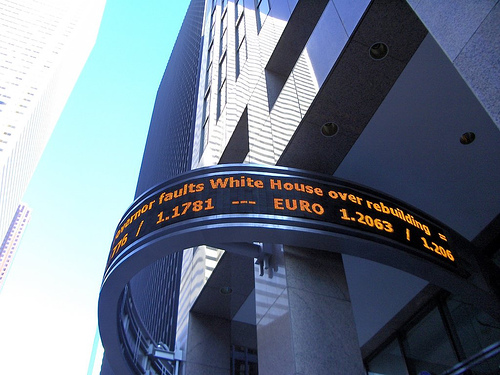
\includegraphics[height=0.50\textheight]{ch1_reuters_ticker.jpg}\\[1mm]
\imgcap{Bandă de știri pe clădirea Reuters, New York}
\imgcredit{https://commons.wikimedia.org/wiki/File:Reuters_News_Ticker.jpg}{Foto: bgilliard (2005); CC BY-SA 2.0; Wikimedia Commons}
\end{column}
\end{columns}
\end{frame}

\begin{frame}{Frecvența datelor}
\itemsize{\small}
\begin{itemize}
    \item \textbf{Date tick}: fiecare tranzacție și cotație
    \begin{itemize}
        \item milioane de înregistrări pe zi; zgomot din saltul între bid și ask
    \end{itemize}
    \item \textbf{Bare intrazilnice}: 1, 5 sau 60 de minute
    \begin{itemize}
        \item folosite pentru volatilitatea realizată (Capitolul 8)
    \end{itemize}
    \item \textbf{Date zilnice}: un rînd pe zi de tranzacționare
    \begin{itemize}
        \item standardul acestui curs și al majorității studiilor academice
        \item bursele funcționează aproximativ 250 de zile pe an; piețele cripto, 365 de zile pe an
    \end{itemize}
    \item \textbf{Date săptămînale, lunare, anuale}
    \begin{itemize}
        \item mai puține observații, mai aproape de orizontul investitorilor pe termen lung
    \end{itemize}
    \item Regulă: anualizați cu numărul \textbf{real} de observații pe an al fiecărei serii
\end{itemize}
\end{frame}

\begin{frame}{De unde vin datele}
\itemsize{\small}
\begin{center}
\footnotesize
\begin{tabular}{>{\raggedright\arraybackslash}p{3.4cm}>{\raggedright\arraybackslash}p{5.6cm}>{\raggedright\arraybackslash}p{3.4cm}}
\toprule
\textbf{Sursa} & \textbf{Date disponibile} & \textbf{Acces} \\
\midrule
Burse (BVB, Deutsche Börse, NYSE) & prețuri oficiale, volume, niveluri ale indicilor & site, fluxuri contra cost \\
Furnizori de date (Bloomberg, LSEG, EODHD) & prețuri de pe multe piețe, prețuri ajustate, date fundamentale & abonament \\
Bănci centrale (BNR, BCE, Rezerva Federală) & cursuri de referință, rate ale dobînzii & gratuit \\
Baze de date statistice (FRED, Eurostat) & serii macroeconomice, randamente ale titlurilor de stat & gratuit \\
Baze de date academice (CRSP, biblioteca Kenneth French) & randamente curățate, inclusiv firme delistate; randamente ale factorilor & licență universitară sau gratuit \\
Burse și agregatoare cripto & prețuri 24/7, date on-chain & gratuit sau abonament \\
\bottomrule
\end{tabular}
\end{center}
\begin{itemize}
    \item Furnizorul colectează și curăță; \textbf{proprietarul} cifrei (bursa, banca centrală) este referința cînd două surse diferă
\end{itemize}
\end{frame}

\begin{frame}{Datele acestui curs}
\itemsize{\small}
\begin{itemize}
    \item Date zilnice de piață de la \textbf{EODHD} (EOD Historical Data), salvate o singură dată în depozitul cursului
    \begin{itemize}
        \item 91 de serii: indici, ETF-uri, acțiuni (BVB, SUA, Europa), cripto, cursuri de schimb, randamente ale obligațiunilor
        \item coloane: data, deschidere, maxim, minim, închidere, închidere ajustată, volum
    \end{itemize}
    \item EUR/RON: cursul oficial de referință al \textbf{BNR}
    \begin{itemize}
        \item seria EUR/RON de la EODHD are cotații eronate (slide-urile următoare)
    \end{itemize}
    \item Convenții
    \begin{itemize}
        \item indici, cursuri de schimb, cripto: \textit{close}; acțiuni și ETF-uri: \textit{adjusted close}
        \item cotațiile de weekend și închiderile repetate în zilele libere se elimină, cu excepția cripto
        \item fiecare serie se analizează pe propriul calendar
    \end{itemize}
    \item Perioada de comparație a capitolului: 1 ianuarie 2015 -- 18 septembrie 2026
\end{itemize}
\end{frame}

\begin{frame}{Barele zilnice: OHLCV}
\itemsize{\footnotesize}
\begin{itemize}
    \item \textbf{OHLCV}: prețul de deschidere $O_t$, maxim $H_t$, minim $L_t$, de închidere $C_t$ și volumul $V_t$ din ziua $t$
    \item Prin construcție $L_t \le O_t, C_t \le H_t$; amplitudinea $H_t - L_t$ măsoară împrăștierea prețurilor în timpul zilei
    \item Banca Transilvania (TLV), ultimele cinci zile de tranzacționare din datele noastre:
\end{itemize}\begin{center}
\footnotesize
\begin{tabular}{lrrrrr}
\toprule
Data & Open & High & Low & Close & Volum \\
\midrule
14 sep. 2026 & $34{,}52$ & $34{,}86$ & $34{,}28$ & $34{,}54$ & 346\,819 \\
15 sep. 2026 & $34{,}40$ & $34{,}68$ & $33{,}10$ & $34{,}00$ & 676\,653 \\
16 sep. 2026 & $34{,}00$ & $34{,}10$ & $33{,}20$ & $33{,}40$ & 853\,078 \\
17 sep. 2026 & $33{,}40$ & $33{,}40$ & $33{,}40$ & $33{,}40$ & 1\,084\,380 \\
18 sep. 2026 & $34{,}22$ & $35{,}80$ & $34{,}22$ & $35{,}50$ & 1\,884\,988 \\
\bottomrule
\end{tabular}
\end{center}
\begin{itemize}
    \item Verificare: pe 17 septembrie 2026 deschidere = maxim = minim = închidere, cu 1\,084\,380 de acțiuni tranzacționate; o bară plată cu volum mare este suspectă
\end{itemize}
\end{frame}

\begin{frame}{Evenimente corporative și prețul ajustat}
\itemsize{\small}
\begin{itemize}
    \item Prețul de închidere $P_t$ sare în ziua unui eveniment corporativ; valoarea deținerii nu sare
    \item \textbf{Factorul de ajustare} $A$ în ziua evenimentului
    \begin{itemize}
        \item dividend în numerar $D$: $A = 1 - D/P_{t-1}$
        \item split $m$-la-$n$ ($m$ acțiuni noi pentru $n$ vechi): $A = n/m$; o consolidare este un split cu $m < n$
    \end{itemize}
    \item \textbf{Prețul ajustat}: fiecare preț anterior se înmulțește cu factorii tuturor evenimentelor ulterioare, $P^{\text{adj}}_t = P_t \prod_{k:\, t_k > t} A_{t_k}$
    \item Randamentele calculate din prețuri ajustate includ dividendul și nu au salturi artificiale
    \item Cu dividende, randamentul simplu este $R_t = (P_t + D_t)/P_{t-1} - 1$ \refFHH
\end{itemize}
\end{frame}

\begin{frame}{Exemplu lucrat: prețuri ajustate}
\itemsize{\small}
\begin{itemize}
    \item O acțiune cotează la 100; în ziua 5 plătește un dividend de 2; în ziua 10 are loc un split 2-la-1
    \item Factorii de ajustare
    \begin{itemize}
        \item dividend: $A_5 = 1 - 2/100 = 0{,}98$; split: $A_{10} = 1/2 = 0{,}50$
    \end{itemize}
    \item Prețurile ajustate
    \begin{itemize}
        \item înainte de ziua 5: $P^{\text{adj}}_t = P_t \times 0{,}49$, deci 100 devine 49
        \item între zilele 5 și 9: $P^{\text{adj}}_t = P_t \times 0{,}50$; din ziua 10: $P^{\text{adj}}_t = P_t$
    \end{itemize}
    \item Seria ajustată se schimbă la fiecare eveniment nou: păstrați întotdeauna data descărcării
    \item Indici: un \textbf{indice de preț} ignoră dividendele; un \textbf{indice de randament total} le reinvestește
\end{itemize}
\end{frame}

\begin{frame}{Date reale: Banca Transilvania, preț de închidere vs preț ajustat}
\itemsize{\footnotesize}
\begin{center}
    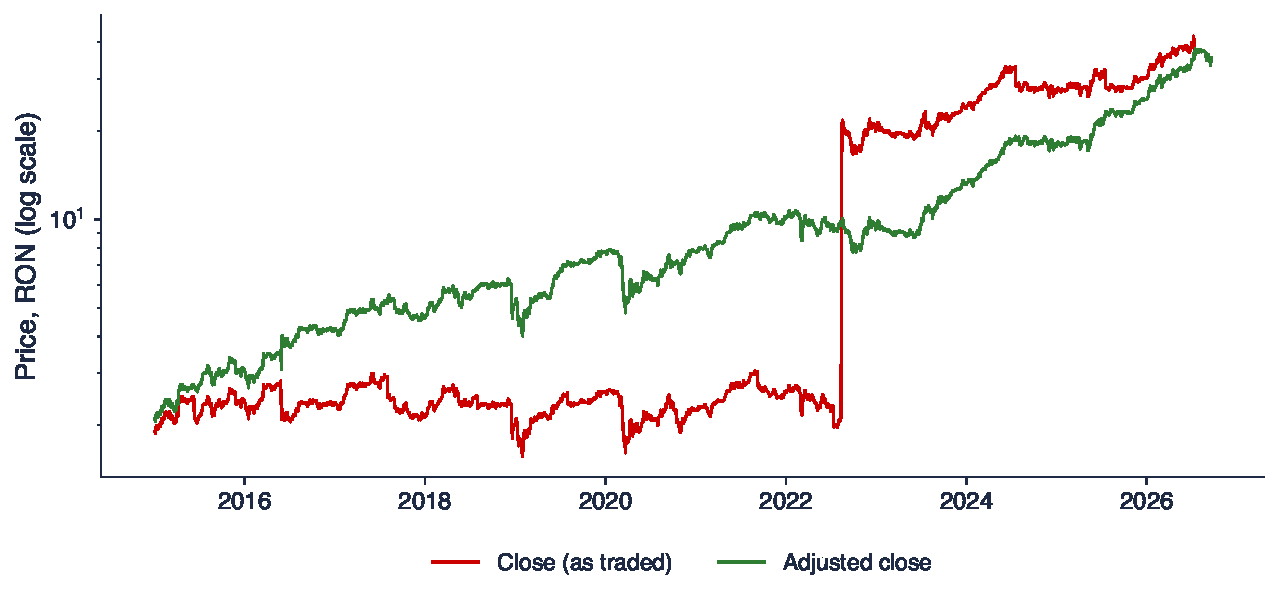
\includegraphics[width=0.97\textwidth,height=0.58\textheight,keepaspectratio]{sfm_ch1_tlv_adjusted.pdf}
\end{center}
\vspace{-0.25cm}
\begin{itemize}
    \item Pe 16 august 2022 prețul sare de la 2{,}12 la 21{,}20 lei: o consolidare a acțiunilor, 10{,}0 acțiuni vechi într-una
    \item Randamentul logaritmic din prețul de închidere: $+230\%$ într-o zi; din prețul ajustat: $0{,}0\%$
    \item Din 2015 cele două serii diferă cu peste 2\% în 24 de zile (dividende, acțiuni gratuite)
\end{itemize}
\quantlet{SFM\_ch1\_data\_quality}{\qlurl{SFM_ch1_data_quality}}
\end{frame}

\begin{frame}{Dividendele contează: BET vs BET-TR}
\itemsize{\footnotesize}
\begin{center}
    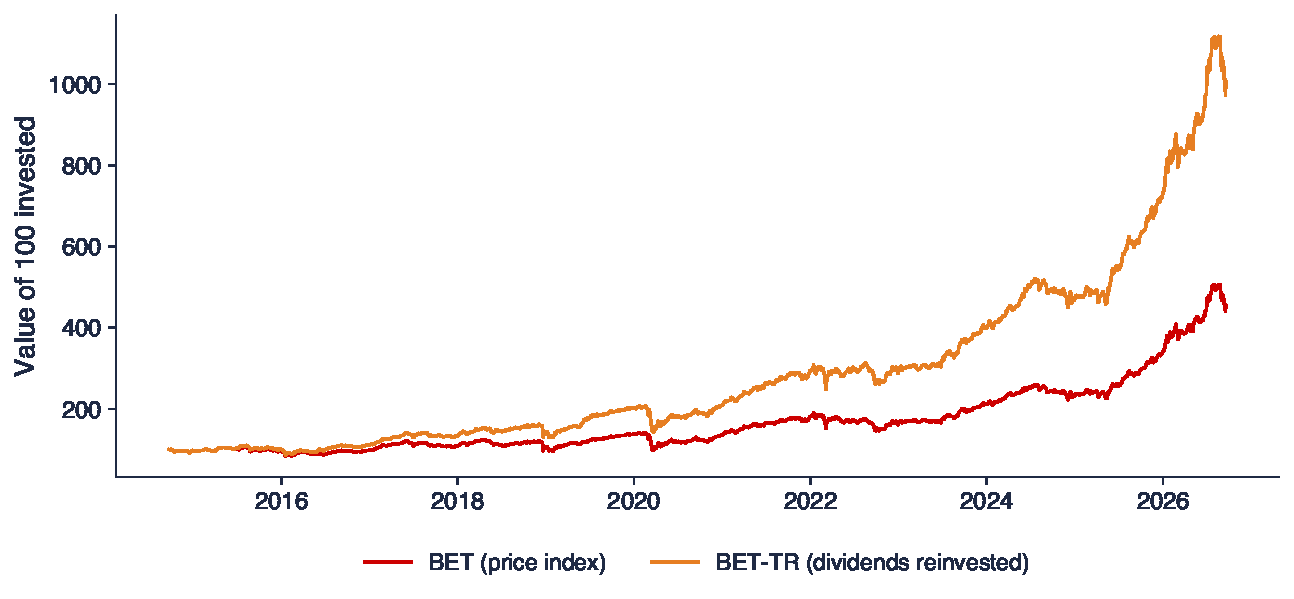
\includegraphics[width=0.97\textwidth,height=0.58\textheight,keepaspectratio]{sfm_ch1_bet_bettr.pdf}
\end{center}
\vspace{-0.25cm}
\begin{itemize}
    \item 100 investiți pe 23 septembrie 2014: 455 în BET (indice de preț), 1005 în BET-TR (dividende reinvestite)
    \item Rata de creștere: 13{,}5\% vs 21{,}2\% pe an; dividendele adaugă 7{,}8 puncte procentuale pe an
    \item Comparați lucruri comparabile: DAX este un indice de randament total, S\&P 500 și BET sînt indici de preț
\end{itemize}
\quantlet{SFM\_ch1\_data\_quality}{\qlurl{SFM_ch1_data_quality}}
\end{frame}

\begin{frame}{Erori în date: două serii EUR/RON}
\itemsize{\footnotesize}
\begin{center}
    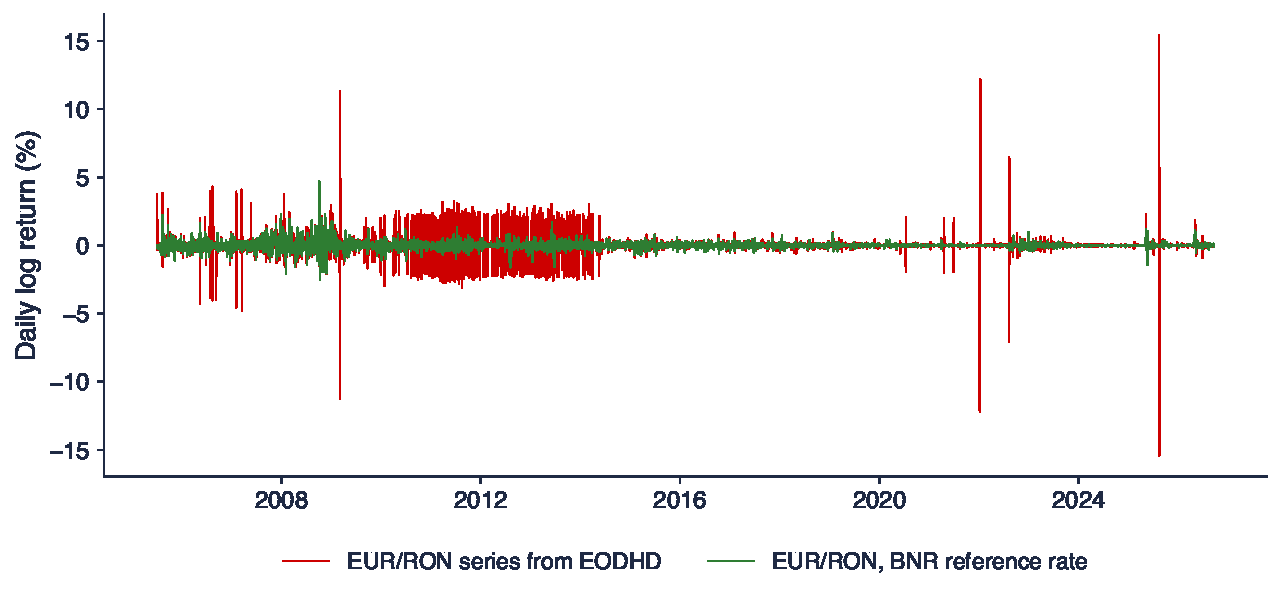
\includegraphics[width=0.97\textwidth,height=0.54\textheight,keepaspectratio]{sfm_ch1_eurron_check.pdf}
\end{center}
\vspace{-0.25cm}
\begin{itemize}
    \item Același curs, 5\,154 de zile comune: seria EODHD se abate cu peste 1 punct procentual de la cursul BNR în 412 de zile
    \item Volatilitatea anualizată: 13{,}4\% (EODHD) vs 4{,}5\% (BNR); cea mai mare mișcare EODHD $15{,}4\%$, pe 14 august 2025
    \item Soluția: folosiți proprietarul oficial al cifrei, cursul de referință BNR
\end{itemize}
\quantlet{SFM\_ch1\_data\_quality}{\qlurl{SFM_ch1_data_quality}}
\end{frame}

\begin{frame}{Trei erori sistematice care fac rezultatele să pară prea bune}
\itemsize{\small}
\begin{itemize}
    \item \textbf{Survivorship bias}: în eșantion apar doar firmele sau fondurile care încă există
    \begin{itemize}
        \item perdanții au dispărut, deci randamentul mediu este prea mare \refBGIR
        \item exemplu: componența actuală a BET, urmărită înapoi pînă în 2000
    \end{itemize}
    \item \textbf{Look-ahead bias}: folosirea unei informații care nu era disponibilă la data deciziei
    \begin{itemize}
        \item rapoarte anuale publicate în martie folosite pentru decizii din ianuarie
    \end{itemize}
    \item \textbf{Data snooping}: încercarea multor reguli pe aceleași date și raportarea celei mai bune
    \begin{itemize}
        \item sute de predictori publicați ai randamentelor sînt probabil descoperiri false \refHLZ
    \end{itemize}
    \item Fiecare eroare umflă randamentele; niciuna nu se vede în statisticile descriptive
\end{itemize}
\end{frame}

\begin{frame}{O listă de verificare a datelor}
\itemsize{\small}
\begin{itemize}
    \item Sursa: cine este proprietarul cifrei și ce coloană (close sau adjusted close) ați folosit?
    \item Calendarul: weekenduri, zile libere, zile lipsă; aceleași date pentru toate activele într-o analiză comună
    \item Salturi: listați cele mai mari 10 randamente în valoare absolută și verificați fiecare cu știrile
    \item Bare plate, volum zero, prețuri repetate: zile libere completate cu ultimul preț sau cotații vechi
    \item Unități și monedă: lei, euro, dolari; puncte de indice; prețuri în cenți
    \item Păstrați fișierul brut și data descărcării; nu modificați niciodată datele manual
\end{itemize}
\end{frame}

\begin{frame}{Recapitulare: Date}
\itemsize{\small}
\begin{itemize}
    \item Prețurile vin de la burse, furnizori și bănci centrale; proprietarul cifrei este referința
    \item Folosiți prețuri ajustate pentru acțiuni și indici de randament total cînd dividendele contează
    \item Datele reale conțin erori: verificați salturile, barele plate și o a doua sursă
    \item Survivorship, look-ahead și data snooping umflă rezultatele fără să se vadă
\end{itemize}
\end{frame}


%=============================================================================
\section{De la prețuri la randamente}
%=============================================================================

\begin{frame}{De ce randamente, nu prețuri?}
\itemsize{\small}
\begin{itemize}
    \item Un preț are unitate de măsură și scară; un randament nu are
    \begin{itemize}
        \item o mișcare de 1 leu este mare pentru o acțiune de 2 lei și mică pentru una de 500 de lei
    \end{itemize}
    \item Randamentele unor active, monede și perioade diferite se pot compara direct
    \item Prețurile au trend și rătăcesc; randamentele oscilează în jurul unui nivel stabil
    \begin{itemize}
        \item serie \textbf{slab staționară}: medie constantă, varianță constantă și o covarianță care depinde doar de decalaj
        \item majoritatea metodelor statistice ale cursului presupun (cel puțin) staționaritate slabă
    \end{itemize}
    \item Investitorul este interesat de variația relativă a averii, adică exact de un randament
\end{itemize}
\end{frame}

\begin{frame}{S\&P 500: nivelul prețului vs randamentele zilnice}
\itemsize{\footnotesize}
\begin{center}
    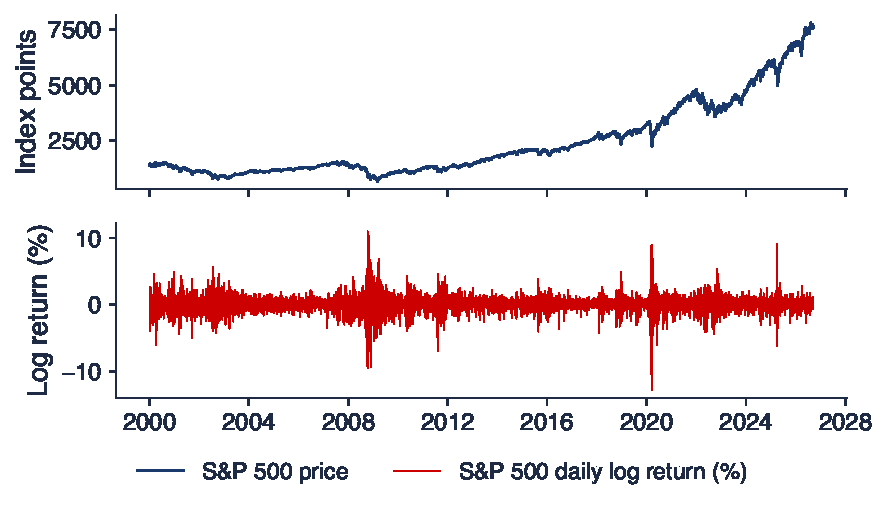
\includegraphics[width=0.97\textwidth,height=0.62\textheight,keepaspectratio]{sfm_ch1_price_returns.pdf}
\end{center}
\vspace{-0.25cm}
\begin{itemize}
    \item Sus: prețul are trend crescător, cu oscilații lungi; media și împrăștierea lui se schimbă în timp
    \item Jos: randamentele oscilează în jurul lui zero, în perioade calme și agitate (2008, 2020)
\end{itemize}
\quantlet{SFM\_ch1\_prices\_returns}{\qlurl{SFM_ch1_prices_returns}}
\end{frame}

\begin{frame}{O verificare formală: testul ADF}
\itemsize{\small}
\begin{itemize}
    \item \textbf{Testul ADF} \refDF: are seria o rădăcină unitară (un mers aleator)?
    \begin{itemize}
        \item $H_0$: rădăcină unitară, nestaționară; $H_1$: staționară
        \item regresia $\Delta y_t = \alpha + \beta t + \gamma y_{t-1} + \sum_j \delta_j \Delta y_{t-j} + \varepsilon_t$; respingem $H_0$ cînd statistica $t$ a lui $\gamma$ este foarte negativă
    \end{itemize}
    \item S\&P 500, date zilnice din 2000
    \begin{itemize}
        \item logaritmul prețului (cu trend): statistica $-2{,}08$, valoarea critică 5\% $-3{,}41$, $p = 0{,}56$: nu respingem rădăcina unitară
        \item randamente logaritmice: statistica $-14{,}3$, valoarea critică 5\% $-2{,}86$, $p < 0{,}001$: o respingem
    \end{itemize}
    \item Rădăcinile unitare și mersul aleator sînt subiectul \sfmchlink{https://danpele.github.io/SFM/RO/Cursuri/capitol7_piete_eficiente_mers_aleator_vr.pdf}{Capitolului 7}
\end{itemize}\quantlet{SFM\_ch1\_prices\_returns}{\qlurl{SFM_ch1_prices_returns}}
\end{frame}


%=============================================================================
\section{Randamente simple și logaritmice}
%=============================================================================

\begin{frame}{Randamentul simplu}
\itemsize{\small}
\begin{itemize}
    \item \textbf{Randamentul simplu (net)} de la $t-1$ la $t$ \refFHH, \refTsay
    \begin{itemize}
        \item $R_t = \dfrac{P_t - P_{t-1}}{P_{t-1}} = \dfrac{P_t}{P_{t-1}} - 1$
        \item \textbf{randamentul brut}: $1 + R_t = P_t / P_{t-1}$
    \end{itemize}
    \item Mărginit inferior: $R_t \ge -1$ (răspundere limitată: nu puteți pierde mai mult decît ați investit)
    \item Exemplu: $P_{t-1} = 100$, $P_t = 110$: $R_t = 10\%$
    \item Este ceea ce vede investitorul în extrasul de cont: „fondul a cîștigat 10\%”
    \item Notație: de aici încolo $P_t$ este prețul de închidere al unui indice sau prețul ajustat al unei acțiuni
\end{itemize}
\end{frame}

\begin{frame}{Randamentul logaritmic}
\itemsize{\small}
\begin{itemize}
    \item \textbf{Randamentul logaritmic} (randamentul compus continuu)
    \begin{itemize}
        \item $r_t = \ln\dfrac{P_t}{P_{t-1}} = \ln P_t - \ln P_{t-1} = \ln(1 + R_t)$
        \item înapoi la randamentul simplu: $R_t = e^{r_t} - 1$
    \end{itemize}
    \item Denumirea: $e^{r}$ este creșterea unui leu la rata $r$, compusă continuu pe durata perioadei
    \item Nemărginit: $r_t \in (-\infty, +\infty)$; pierderea totală ($P_t = 0$) înseamnă $r_t = -\infty$
    \item Exemplu: $P_{t-1} = 100$, $P_t = 110$: $r_t = \ln 1{,}1 = 9{,}53\%$
    \item Randamentele logaritmice sînt standardul în statistica piețelor financiare: se adună în timp (secțiunea următoare)
\end{itemize}
\end{frame}

\begin{frame}{Cît de departe sînt $r$ și $R$?}
\itemsize{\small}
\begin{itemize}
    \item Dezvoltarea în serie Taylor a logaritmului în jurul lui 0
    \begin{itemize}
        \item $r = \ln(1 + R) = R - \dfrac{R^2}{2} + \dfrac{R^3}{3} - \dots$
        \item $\ln$ este concavă, deci $r < R$ pentru orice $R \neq 0$
    \end{itemize}
    \item Mișcare zilnică, $R = 1\%$
    \begin{itemize}
        \item $r = 0{,}995\%$, iar $R - R^2/2 = 0{,}995\%$: diferența este de 0{,}5 puncte de bază
    \end{itemize}
    \item Mișcare mare, $R = 10\%$
    \begin{itemize}
        \item $r = 9{,}531\%$, iar $R - R^2/2 = 9{,}500\%$: diferența este de 46{,}9 puncte de bază
    \end{itemize}
    \item Un \textbf{punct de bază} (bp) este 0,01 puncte procentuale
    \item Concluzie: pentru randamente zilnice $r \approx R$; pentru mișcări mari și orizonturi lungi diferă
\end{itemize}
\end{frame}

\begin{frame}{Randamente simple vs logaritmice pe extreme reale}
\itemsize{\footnotesize}
\begin{columns}[T]
\begin{column}{0.56\textwidth}
\begin{center}
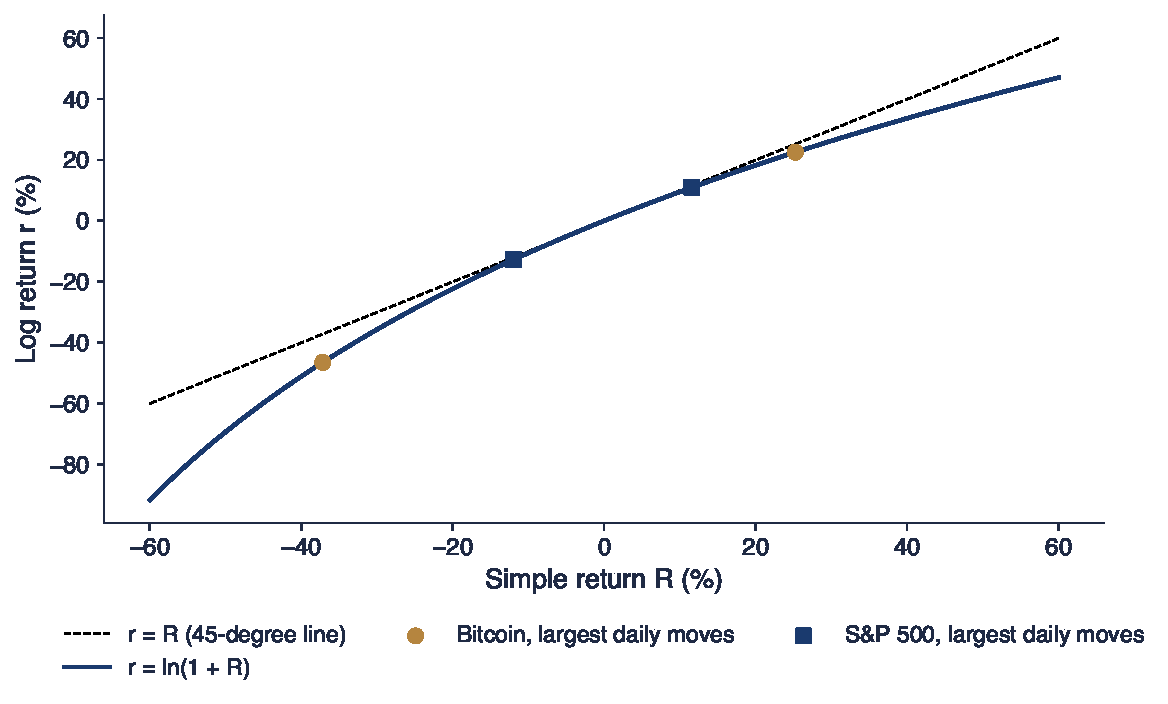
\includegraphics[width=\linewidth,height=0.80\textheight,keepaspectratio]{sfm_ch1_simple_log.pdf}
\end{center}
\end{column}
\begin{column}{0.40\textwidth}
\begin{itemize}
    \item Bitcoin, 12 martie 2020: $R = -37{,}2\%$, dar $r = -46{,}5\%$
    \item Bitcoin, 7 decembrie 2017: $R = +25{,}2\%$, $r = +22{,}5\%$
    \item S\&P 500, 16 martie 2020: $R = -12{,}0\%$, $r = -12{,}8\%$
    \item Curba se îndoaie în jos: pierderile par mai mari, iar cîștigurile mai mici în randamente logaritmice
\end{itemize}
\end{column}
\end{columns}
\quantlet{SFM\_ch1\_simple\_log\_returns}{\qlurl{SFM_ch1_simple_log_returns}}
\end{frame}

\begin{frame}{Exemplu lucrat: +10\%, apoi --10\%}
\itemsize{\small}
\begin{columns}[T]
\begin{column}{0.58\textwidth}
\begin{itemize}
    \item Traiectoria prețului $100 \to 110 \to 99$
    \begin{itemize}
        \item randamente simple: $+10\%$ și $-10\%$; suma lor, 0, este înșelătoare
        \item compuse: $1{,}1 \times 0{,}9 - 1 = -1{,}0\%$
    \end{itemize}
    \item Randamente logaritmice
    \begin{itemize}
        \item $r_1 = \ln 1{,}1 = 9{,}53\%$, $r_2 = \ln 0{,}9 = -10{,}54\%$
        \item suma: $-1{,}01\% = \ln(99/100)$, exact
    \end{itemize}
\end{itemize}
\end{column}
\begin{column}{0.38\textwidth}
\begin{block}{Regula}
\begin{itemize}
    \item Randamentele simple se compun (se înmulțesc); cele logaritmice se adună
\end{itemize}
\end{block}
\end{column}
\end{columns}
\end{frame}

\begin{frame}{Întrebare pentru sală: +50\%, apoi --50\%}
\itemsize{\small}
\begin{itemize}
    \item O acțiune crește cu 50\% într-un an și scade cu 50\% în anul următor
    \item \textbf{Ce credeți?} Unde este prețul după doi ani, față de început?
    \item \textbf{Răspuns}
    \begin{itemize}
        \item $1{,}5 \times 0{,}5 = 0{,}75$: averea s-a modificat cu $-25\%$
        \item randamente logaritmice: $\ln 1{,}5 + \ln 0{,}5 = \ln 0{,}75 = -28{,}8\%$
        \item o pierdere $x$ cere un cîștig de $x/(1-x)$ pentru recuperare: 50\% cere 100\%
    \end{itemize}
\end{itemize}
\end{frame}

\begin{frame}{Ce randament și cînd?}
\itemsize{\small}
\begin{center}
\footnotesize
\begin{tabular}{>{\raggedright\arraybackslash}p{4.2cm}>{\raggedright\arraybackslash}p{2.6cm}>{\raggedright\arraybackslash}p{5.6cm}}
\toprule
\textbf{Situația} & \textbf{Folosiți} & \textbf{Motivul} \\
\midrule
Agregarea în timp & logaritmic & $r_{t}(k) = r_t + \dots + r_{t-k+1}$, o sumă \\
Portofoliu din mai multe active & simplu & $R_p = \sum_i w_i R_i$, exact \\
Modelare statistică & logaritmic & nemărginit, mai aproape de o distribuție simetrică \\
Raportare către investitori & simplu & „fondul a cîștigat 10\%” este un randament simplu \\
Date zilnice, mișcări mici & oricare & diferența este aproximativ $R^2/2$ \\
\bottomrule
\end{tabular}
\end{center}
\begin{itemize}
    \item Spuneți întotdeauna pe care îl folosiți: un „randament de 10\%” este ambiguu
\end{itemize}
\end{frame}

\begin{frame}{Recapitulare: Randamente simple și logaritmice}
\itemsize{\small}
\begin{itemize}
    \item $R_t = P_t/P_{t-1} - 1$; $r_t = \ln(P_t/P_{t-1}) = \ln(1 + R_t)$
    \item $r < R$ pentru orice mișcare; diferența este aproximativ $R^2/2$, neglijabilă pentru date zilnice
    \item Randamentele logaritmice se adună în timp; cele simple se adună între active
    \item Cîștigurile și pierderile de aceeași mărime nu se anulează
\end{itemize}
\end{frame}


%=============================================================================
\section{Randamente pe mai multe perioade și ale portofoliilor}
%=============================================================================

\begin{frame}{Randamente pe $k$ perioade}
\itemsize{\small}
\begin{itemize}
    \item \textbf{Simple}: randamentele brute se înmulțesc
    \begin{itemize}
        \item $1 + R_t(k) = \dfrac{P_t}{P_{t-k}} = (1 + R_t)(1 + R_{t-1}) \cdots (1 + R_{t-k+1})$
    \end{itemize}
    \item \textbf{Logaritmice}: randamentele se adună
    \begin{itemize}
        \item $r_t(k) = \ln\dfrac{P_t}{P_{t-k}} = r_t + r_{t-1} + \dots + r_{t-k+1}$
    \end{itemize}
    \item Consecință: media și varianța randamentului logaritmic pe $k$ zile rezultă din cele ale randamentelor zilnice
    \item Randamentele săptămînale, lunare sau anuale se calculează din prețurile de la sfîrșitul fiecărei perioade, nu prin mediere
\end{itemize}
\end{frame}

\begin{frame}{Randamentul cumulat și averea}
\itemsize{\small}
\begin{itemize}
    \item Averea după $T$ perioade, pornind de la $W_0$: $W_T = W_0 \prod_{t=1}^{T} (1 + R_t) = W_0 \exp\Big(\sum_{t=1}^{T} r_t\Big)$
    \item \textbf{Randamentul simplu cumulat}: $\text{CSR}_T = W_T/W_0 - 1$
    \begin{itemize}
        \item ce a cîștigat investitorul, în procente
    \end{itemize}
    \item \textbf{Randamentul logaritmic cumulat}: $\text{CLR}_T = \ln(W_T/W_0) = \sum_t r_t$
    \begin{itemize}
        \item legătura: $\text{CSR}_T = e^{\text{CLR}_T} - 1$
    \end{itemize}
    \item Scara logaritmică pe grafice: distanțe verticale egale înseamnă variații procentuale egale
\end{itemize}
\end{frame}

\begin{frame}{Creșterea a 100 investiți, 2015--2026}
\itemsize{\footnotesize}
\begin{center}
    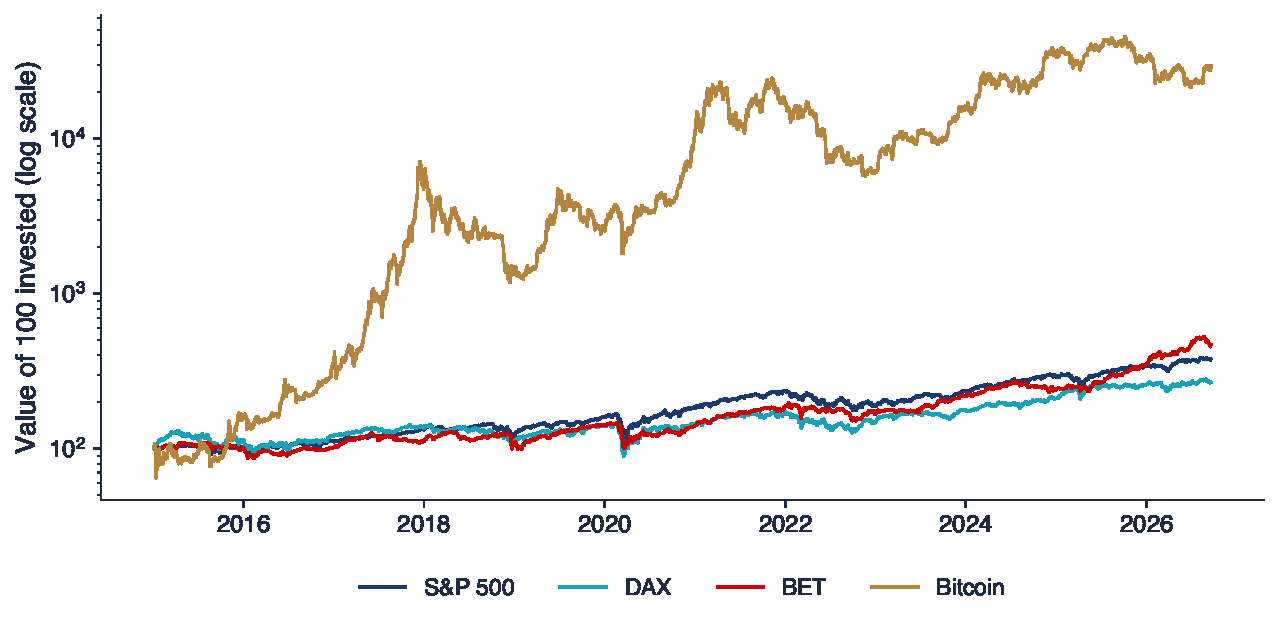
\includegraphics[width=0.97\textwidth,height=0.58\textheight,keepaspectratio]{sfm_ch1_growth.pdf}
\end{center}
\vspace{-0.25cm}
\begin{itemize}
    \item Valori finale: S\&P 500 379, DAX 267, BET 470, Bitcoin 29475
    \item Bitcoin: randament simplu cumulat 29375\%, randament logaritmic cumulat 5{,}69; BET: 370\% și 1{,}55
    \item Fără scara logaritmică, toate seriile, mai puțin Bitcoin, ar părea plate
\end{itemize}
\quantlet{SFM\_ch1\_portfolio\_returns}{\qlurl{SFM_ch1_portfolio_returns}}
\end{frame}

\begin{frame}{Randamentul unui portofoliu}
\itemsize{\small}
\begin{itemize}
    \item Portofoliu cu ponderile $w_1, \dots, w_n$, $\sum_i w_i = 1$, fixate la începutul perioadei
    \begin{itemize}
        \item \textbf{simplu}: $R_p = \sum_i w_i R_i$, exact
        \item \textbf{logaritmic}: $r_p = \ln\big(\sum_i w_i e^{r_i}\big) \neq \sum_i w_i r_i$
    \end{itemize}
    \item Exemplu: 60\% în A ($R_A = 10\%$), 40\% în B ($R_B = -5\%$)
    \begin{itemize}
        \item $R_p = 0{,}6 \times 10\% + 0{,}4 \times (-5\%) = 4{,}0\%$; exact $r_p = \ln(1 + R_p) = 3{,}92\%$
        \item randamente logaritmice ponderate: $0{,}6 \times 9{,}53\% + 0{,}4 \times (-5{,}13\%) = 3{,}67\%$, prea mic
    \end{itemize}
    \item Ponderile se modifică atunci cînd prețurile se mișcă: un portofoliu cu ponderi fixe trebuie \textbf{reechilibrat}
\end{itemize}\quantlet{SFM\_ch1\_portfolio\_returns}{\qlurl{SFM_ch1_portfolio_returns}}
\end{frame}

\begin{frame}{Date reale: un portofoliu TLV--SNP}
\itemsize{\small}
\begin{itemize}
    \item 50\% Banca Transilvania, 50\% OMV Petrom, reechilibrat zilnic, 2015--2026
    \item O zi: randamentul logaritmic exact vs suma ponderată a randamentelor logaritmice
    \begin{itemize}
        \item diferența medie în valoare absolută 0{,}38 puncte de bază; cea mai mare 13{,}9 puncte de bază, pe 31 mai 2016
    \end{itemize}
    \item Pe întreaga perioadă diferențele mici se acumulează
    \begin{itemize}
        \item randamentul logaritmic cumulat exact 2{,}56, deci 1 leu devine 13{,}0 lei
        \item randamentele logaritmice ponderate dau 2{,}47, deci doar 11{,}8 lei
    \end{itemize}
    \item Rata de creștere: portofoliul 24{,}5\% pe an; TLV 27{,}3\%; SNP 19{,}7\%
    \item Regula: construiți portofoliile cu randamente simple, apoi logaritmați dacă e nevoie
\end{itemize}\quantlet{SFM\_ch1\_portfolio\_returns}{\qlurl{SFM_ch1_portfolio_returns}}
\end{frame}

\begin{frame}{Recapitulare: Randamente pe mai multe perioade și ale portofoliilor}
\itemsize{\small}
\begin{itemize}
    \item În timp: înmulțiți randamentele brute sau adunați randamentele logaritmice
    \item Averea $W_T = W_0 e^{\text{CLR}_T}$; $\text{CSR}_T = e^{\text{CLR}_T} - 1$
    \item Între active: $R_p = \sum_i w_i R_i$ exact; varianta logaritmică este doar o aproximare
    \item Erorile mici zilnice de aproximare devin vizibile pe un deceniu
\end{itemize}
\end{frame}


%=============================================================================
\section{Anualizarea}
%=============================================================================

\begin{frame}{Anualizarea mediei și a volatilității}
\itemsize{\small}
\begin{itemize}
    \item $q$ = numărul de observații pe an: aproximativ 252 pentru burse, 365 pentru cripto, 52 pentru date săptămînale, 12 pentru date lunare
    \item \textbf{Media}: randamentele logaritmice se adună, deci $\mu_{\text{an}} = q\,\mu$
    \begin{itemize}
        \item aceeași regulă se folosește pentru media randamentelor simple (anualizare aritmetică)
    \end{itemize}
    \item \textbf{Volatilitatea} = abaterea standard a randamentelor: $\sigma_{\text{an}} = \sqrt{q}\,\sigma$, \textbf{regula rădăcinii pătrate a timpului}
    \begin{itemize}
        \item valabilă cînd randamentele sînt necorelate și au varianță constantă: atunci $\Var(r_1 + \dots + r_q) = q\,\sigma^2$
    \end{itemize}
    \item S\&P 500: $\sigma$ zilnic $= 1{,}12\%$, deci $\sigma_{\text{an}} = 1{,}12\% \times 15{,}87 = 17{,}7\%$
    \begin{itemize}
        \item Bitcoin: $\sqrt{365} = 19{,}10$ dă 66{,}6\%; factorul bursier $\sqrt{252}$ ar da doar 55{,}4\%
    \end{itemize}
\end{itemize}
\end{frame}

\begin{frame}{Rata anuală compusă de creștere}
\itemsize{\small}
\begin{itemize}
    \item \textbf{CAGR} (compound annual growth rate, rata anuală compusă de creștere): rata anuală constantă care transformă $P_0$ în $P_T$ în $Y$ ani
    \begin{itemize}
        \item $\text{CAGR} = \big(P_T / P_0\big)^{1/Y} - 1$, cu $Y$ în ani calendaristici
    \end{itemize}
    \item Legătura cu randamentele logaritmice: $\text{CAGR} = \exp(\text{media anuală a randamentelor logaritmice}) - 1$
    \item S\&P 500, 2015--2026: media randamentelor logaritmice 11{,}2\% pe an, $e^{11{,}2\%} - 1 = 11{,}9\%$, iar CAGR este 11{,}9\%
    \item CAGR folosește doar primul și ultimul preț: nu spune nimic despre traiectoria dintre ele
    \item Se mai numește randamentul mediu geometric
\end{itemize}
\end{frame}

\begin{frame}{Cît de precis cunoaștem media?}
\itemsize{\small}
\begin{itemize}
    \item Eroarea standard a mediei anuale: $\text{SE}(\hat\mu_{\text{an}}) = \sigma_{\text{an}} / \sqrt{Y}$, cu $Y$ ani de date
    \begin{itemize}
        \item depinde de numărul de \textbf{ani}, nu de numărul de observații
    \end{itemize}
    \item S\&P 500, 11{,}7 ani: media anuală a randamentelor logaritmice 11{,}2\%, SE 5{,}2\%
    \begin{itemize}
        \item CI 95\% (confidence interval, interval de încredere): [1{,}1\%, 21{,}4\%]
    \end{itemize}
    \item Bitcoin: 47{,}4\% $\pm$ $1{,}96 \times 19{,}5\%$
    \begin{itemize}
        \item intervalul este [9{,}2\%, 85{,}6\%]: foarte larg
    \end{itemize}
    \item Volatilitatea, în schimb, se estimează precis din date zilnice
\end{itemize}\quantlet{SFM\_ch1\_descriptive\_stats}{\qlurl{SFM_ch1_descriptive_stats}}
\end{frame}

\begin{frame}{Întrebare pentru sală: mai multe date, o medie mai bună?}
\itemsize{\small}
\begin{itemize}
    \item Înlocuiți 10 ani de date zilnice S\&P 500 cu 10 ani de date la 5 minute: 78 de bare într-o zi de tranzacționare de 6,5 ore, deci de 78 de ori mai multe observații
    \item \textbf{Ce credeți?} Devine mai mică eroarea standard a randamentului mediu anual?
    \item \textbf{Răspuns}
    \begin{itemize}
        \item Nu: media pe 10 ani este fixată de primul și ultimul preț, $\hat\mu = \ln(P_T/P_0)/Y$
        \item doar mai mulți \textbf{ani} îi reduc eroarea standard, ca $1/\sqrt{Y}$
        \item estimarea volatilității, în schimb, se îmbunătățește cu frecvența
    \end{itemize}
\end{itemize}
\end{frame}

\begin{frame}{Recapitulare: Anualizarea}
\itemsize{\small}
\begin{itemize}
    \item Media $\times\, q$, volatilitatea $\times \sqrt{q}$, cu $q$ numărul real de observații pe an
    \item $\sqrt{q}$ presupune randamente necorelate, cu varianță constantă
    \item CAGR $= (P_T/P_0)^{1/Y} - 1$, exponențiala mediei anuale a randamentelor logaritmice minus 1
    \item Mediile randamentelor sînt imprecise: SE $= \sigma_{\text{an}}/\sqrt{Y}$
\end{itemize}
\end{frame}


%=============================================================================
\section{Statisticile descriptive ale randamentelor}
%=============================================================================

\begin{frame}{Poziție și împrăștiere}
\itemsize{\small}
\begin{itemize}
    \item Eșantion $r_1, \dots, r_n$ de randamente logaritmice zilnice (în \%)
    \item \textbf{Media}: $\bar r = \frac1n \sum_{t=1}^{n} r_t$, randamentul zilnic mediu
    \item \textbf{Varianța}: $\hat\sigma^2 = \frac{1}{n-1} \sum_{t=1}^{n} (r_t - \bar r)^2$; \textbf{abaterea standard} $\hat\sigma = \sqrt{\hat\sigma^2}$
    \begin{itemize}
        \item în finanțe abaterea standard a randamentelor se numește \textbf{volatilitate}
    \end{itemize}
    \item \textbf{Cuantila} $q_\alpha$: valoarea sub care se află o fracție $\alpha$ din randamente
    \begin{itemize}
        \item mediana $q_{0{,}5}$; cuantila de 1\% $q_{0{,}01}$ stă la baza VaR 1\% (Capitolul 10)
    \end{itemize}
    \item \textbf{Minimul} și \textbf{maximul}: cea mai proastă și cea mai bună zi, întotdeauna cu datele lor
\end{itemize}
\end{frame}

\begin{frame}{Forma: asimetria și aplatizarea}
\itemsize{\small}
\begin{itemize}
    \item \textbf{Asimetria} (skewness): $\hat S = \frac1n \sum_t (r_t - \bar r)^3 / \hat\sigma^3$
    \begin{itemize}
        \item $S = 0$: simetrică; $S < 0$: coadă stîngă mai lungă, pierderile mari mai frecvente decît cîștigurile mari
    \end{itemize}
    \item \textbf{Aplatizarea} (kurtosis): $\hat K = \frac1n \sum_t (r_t - \bar r)^4 / \hat\sigma^4$; \textbf{excesul de aplatizare} (excess kurtosis) $\hat K - 3$
    \begin{itemize}
        \item distribuția Normală are $K = 3$, deci exces de aplatizare 0
        \item exces de aplatizare $> 0$: \textbf{cozi groase}, zile extreme mai frecvente decît sub distribuția Normală
    \end{itemize}
    \item Ambele sînt sensibile la zile extreme izolate: raportați-le împreună cu extremele
    \item Cozile groase și asimetria sînt \textbf{fapte stilizate} ale randamentelor \refCont; testele formale în \sfmchlink{https://danpele.github.io/SFM/RO/Cursuri/capitol2_distributii_clasice_fapte_stilizate.pdf}{Capitolul 2}
\end{itemize}
\end{frame}

\begin{frame}{Randamente logaritmice zilnice: indici și Bitcoin, 2015--2026}
\itemsize{\small}
\begin{center}
\footnotesize
\begin{tabular}{lrrrrlr}
\toprule
Seria & Media & Abaterea std. & Asim. & Exces aplat. & Minimul (data) & Maximul \\
\midrule
S\&P 500 & $0{,}045$ & $1{,}12$ & $-0{,}64$ & $15{,}8$ & $-12{,}8$ (16 mar. 2020) & $9{,}1$ \\
DAX & $0{,}032$ & $1{,}20$ & $-0{,}56$ & $10{,}0$ & $-13{,}1$ (12 mar. 2020) & $10{,}4$ \\
BET & $0{,}053$ & $0{,}98$ & $-1{,}41$ & $17{,}8$ & $-11{,}9$ (19 dec. 2018) & $6{,}8$ \\
BET-TR & $0{,}080$ & $0{,}98$ & $-1{,}43$ & $18{,}1$ & $-11{,}9$ (19 dec. 2018) & $6{,}7$ \\
Bitcoin & $0{,}130$ & $3{,}49$ & $-0{,}73$ & $12{,}2$ & $-46{,}5$ (12 mar. 2020) & $22{,}5$ \\
\bottomrule
\end{tabular}
\end{center}
\begin{itemize}
    \item Toate valorile în \%, cu excepția asimetriei și a excesului de aplatizare; fiecare serie pe calendarul ei
    \item Bitcoin: abaterea standard zilnică de aproximativ trei ori mai mare decît a indicilor bursieri
    \item Toate seriile: asimetrie negativă și exces de aplatizare mare
    \item Cele mai proaste zile se concentrează în martie 2020 (COVID-19) și pe 19 decembrie 2018 pentru BET
\end{itemize}\quantlet{SFM\_ch1\_descriptive\_stats}{\qlurl{SFM_ch1_descriptive_stats}}
\end{frame}

\begin{frame}{Randamente logaritmice zilnice: cinci acțiuni BVB, 2015--2026}
\itemsize{\small}
\begin{center}
\footnotesize
\begin{tabular}{lrrrrlr}
\toprule
Seria & Media & Abaterea std. & Asim. & Exces aplat. & Minimul (data) & Maximul \\
\midrule
Banca Transilvania (TLV) & $0{,}106$ & $1{,}69$ & $-0{,}55$ & $25{,}2$ & $-22{,}2$ (19 dec. 2018) & $20{,}5$ \\
OMV Petrom (SNP) & $0{,}079$ & $1{,}54$ & $-0{,}66$ & $9{,}2$ & $-15{,}0$ (9 mar. 2020) & $10{,}0$ \\
BRD & $0{,}075$ & $1{,}61$ & $-0{,}51$ & $9{,}2$ & $-18{,}2$ (19 dec. 2018) & $10{,}3$ \\
Nuclearelectrica (SNN) & $0{,}118$ & $1{,}53$ & $0{,}29$ & $5{,}2$ & $-9{,}4$ (9 mar. 2020) & $11{,}3$ \\
Transgaz (TGN) & $0{,}091$ & $1{,}55$ & $0{,}01$ & $5{,}3$ & $-10{,}1$ (19 dec. 2018) & $11{,}1$ \\
\bottomrule
\end{tabular}
\end{center}
\begin{itemize}
    \item Acțiunile individuale sînt mai volatile decît indicele BET: efectul diversificării
    \item Banca Transilvania și BRD au pierdut cel mai mult pe 19 decembrie 2018, după anunțarea taxei pe activele bancare, adoptată prin OUG 114/2018
    \item Excesul de aplatizare diferă mult între acțiuni: comparați TLV cu SNN
    \item Crahurile de la BVB au o statistică proprie \refPele
\end{itemize}\quantlet{SFM\_ch1\_descriptive\_stats}{\qlurl{SFM_ch1_descriptive_stats}}
\end{frame}

\begin{frame}{Histograme vs distribuția Normală}
\itemsize{\footnotesize}
\begin{center}
    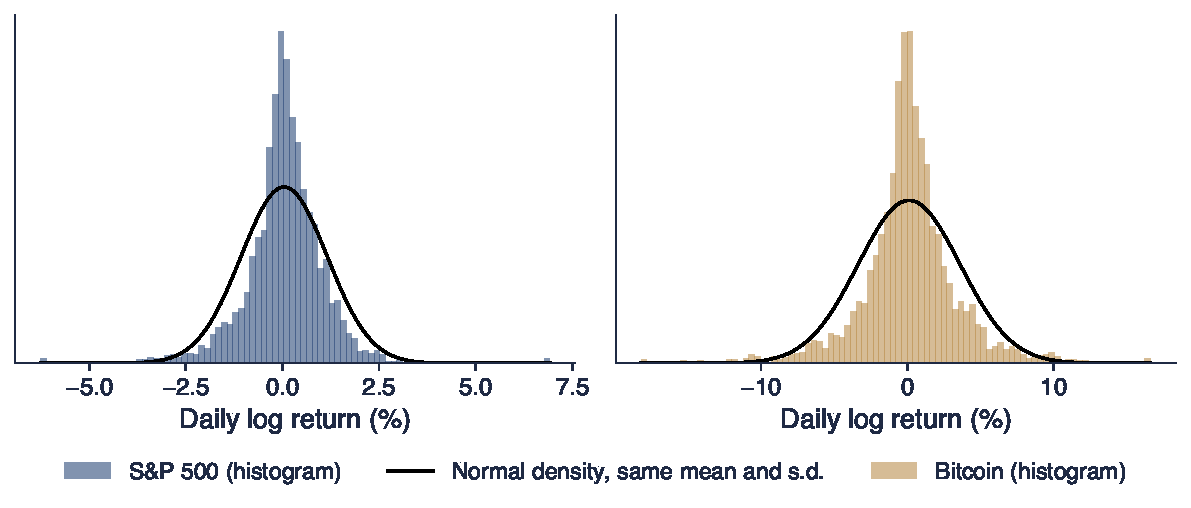
\includegraphics[width=0.97\textwidth,height=0.55\textheight,keepaspectratio]{sfm_ch1_hist_normal.pdf}
\end{center}
\vspace{-0.25cm}
\begin{itemize}
    \item Linia neagră: densitatea Normală cu aceeași medie și abatere standard
    \item S\&P 500: 79{,}6\% din zile sînt la cel mult o abatere standard de medie (distribuția Normală: 68{,}3\%)
    \item Dincolo de trei abateri standard: 1{,}39\% din zile vs 0{,}27\% sub distribuția Normală, de 5{,}2 ori mai multe
\end{itemize}
\quantlet{SFM\_ch1\_descriptive\_stats}{\qlurl{SFM_ch1_descriptive_stats}}
\end{frame}

\begin{frame}{Volatilitatea se schimbă în timp}
\itemsize{\footnotesize}
\begin{center}
    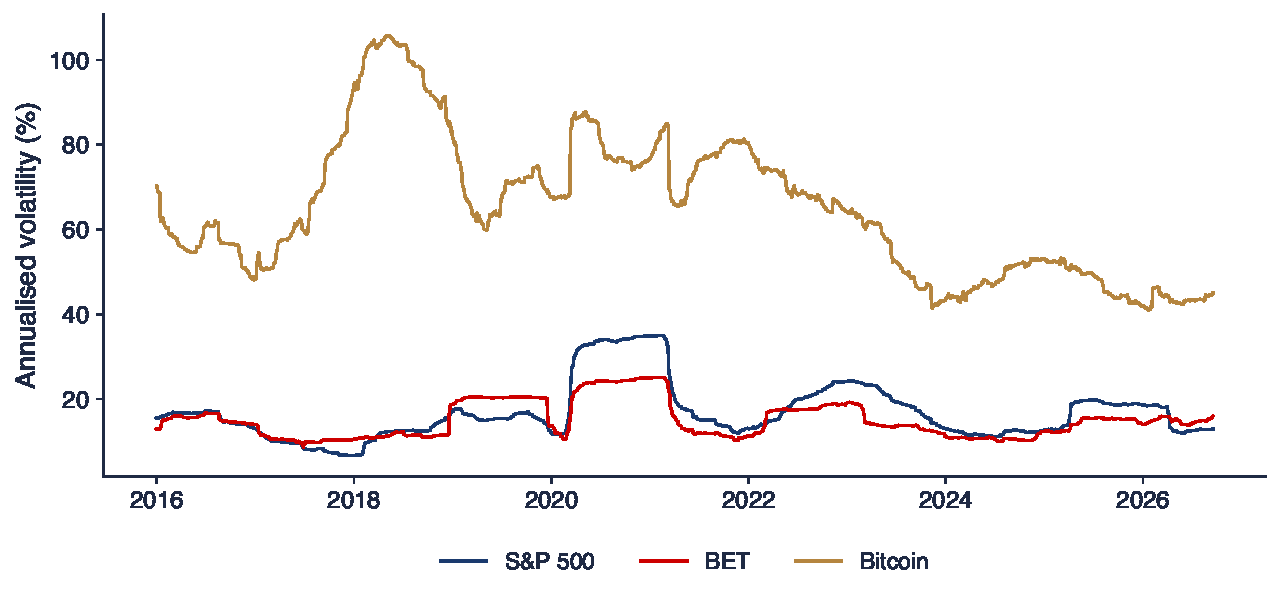
\includegraphics[width=0.97\textwidth,height=0.55\textheight,keepaspectratio]{sfm_ch1_rolling_vol_1y.pdf}
\end{center}
\vspace{-0.25cm}
\begin{itemize}
    \item Volatilitatea pe ferestre mobile de un an, anualizată: S\&P 500 între 7\% și 35\%; Bitcoin între 41\% și 106\%
    \item O singură cifră pentru tot eșantionul ascunde perioadele calme și pe cele agitate
    \item Estimatori de volatilitate și modele GARCH: Capitolele 8 și 9
\end{itemize}
\quantlet{SFM\_ch1\_descriptive\_stats}{\qlurl{SFM_ch1_descriptive_stats}}
\end{frame}

\begin{frame}{Recapitulare: Statistici descriptive}
\itemsize{\small}
\begin{itemize}
    \item Raportați media, abaterea standard, asimetria, excesul de aplatizare, cuantilele și extremele cu datele lor
    \item Randamente zilnice: medie apropiată de 0, volatilitate 1--3\% pe zi, cozi groase, adesea asimetrie negativă
    \item Zilele extreme sînt de cîteva ori mai frecvente decît sub distribuția Normală
    \item Volatilitatea nu este constantă în timp
\end{itemize}
\end{frame}


%=============================================================================
\section{Indicatori de performanță}
%=============================================================================

\begin{frame}{De ce o singură cifră nu ajunge}
\itemsize{\small}
\begin{itemize}
    \item Randamentul singur răsplătește asumarea de risc: un pariu cu efect de levier poate arăta un randament mare ani la rînd
    \item Trei întrebări pe care le pune un investitor
    \begin{itemize}
        \item cît a crescut? (CAGR)
        \item cît de agitat a fost drumul? (volatilitate, abaterea negativă)
        \item cît de adîncă a fost cea mai mare cădere și cît a durat recuperarea? (maximum drawdown)
    \end{itemize}
    \item Indicatorii \textbf{ajustați la risc} împart un randament la o măsură a riscului: Sharpe, Sortino, Calmar
    \item Toate sînt estimări dintr-un singur eșantion: fiecare are o eroare de estimare
\end{itemize}
\end{frame}

\begin{frame}{Sharpe ratio}
\itemsize{\small}
\begin{columns}[T]
\begin{column}{0.64\textwidth}
\begin{itemize}
    \item \textbf{Sharpe ratio} \refSharpeA, \refSharpeB: randamentul în exces pe unitatea de risc total
    \begin{itemize}
        \item $\text{SR} = \dfrac{\mu - r_f}{\sigma}$; $\mu$ randamentul mediu, $r_f$ rata fără risc, $\sigma$ volatilitatea
        \item de la zilnic la anual: $\text{SR}_{\text{an}} = \sqrt{q}\,\text{SR}_{\text{zi}}$
    \end{itemize}
    \item Aici: media randamentelor simple zilnice, $r_f = 0$
    \begin{itemize}
        \item activele sînt în lei, euro și dolari, fiecare cu propria rată fără risc
        \item S\&P 500: SR zilnic $0{,}046$, SR anual $0{,}72$
    \end{itemize}
    \item Același Sharpe ratio, același randament pe unitatea de risc, oricare ar fi efectul de levier
\end{itemize}
\end{column}
\begin{column}{0.32\textwidth}
\centering

\includegraphics[height=0.55\textheight]{ch1_sharpe_2007.jpg}\\[1mm]
\imgcap{William F. Sharpe, Premiul Nobel pentru economie 1990}
\imgcredit{https://commons.wikimedia.org/wiki/File:William_sharpe_2007.jpg}{Foto: Larry D. Moore (2007); CC BY 4.0; Wikimedia Commons}
\end{column}
\end{columns}
\end{frame}

\begin{frame}{Sharpe ratio este o estimare}
\itemsize{\small}
\begin{itemize}
    \item Eroarea standard pentru randamente i.i.d. (independente și identic distribuite) \refLo
    \begin{itemize}
        \item $\text{SE}(\widehat{\text{SR}}) \approx \sqrt{(1 + \text{SR}^2/2)/n}$ pe perioadă; anual: înmulțiți cu $\sqrt{q}$
        \item aproximativ $1/\sqrt{Y}$ pentru Sharpe ratio anual: circa $0{,}3$ cu 12 ani de date
    \end{itemize}
    \item S\&P 500, 2015--2026: $\text{SR} = 0{,}72$, SE $0{,}29$
    \begin{itemize}
        \item CI 95\% [$0{,}15$, $1{,}30$]
    \end{itemize}
    \item Cozile groase și gruparea volatilității fac eroarea reală mai mare decît această formulă
    \item Alegerea celei mai bune dintre multe strategii umflă Sharpe ratio al cîștigătoarei \refDSR
\end{itemize}\quantlet{SFM\_ch1\_performance}{\qlurl{SFM_ch1_performance}}
\end{frame}

\begin{frame}{Sharpe ratio cu intervale de 95\%, 2015--2026}
\itemsize{\footnotesize}
\begin{columns}[T]
\begin{column}{0.58\textwidth}
\begin{center}
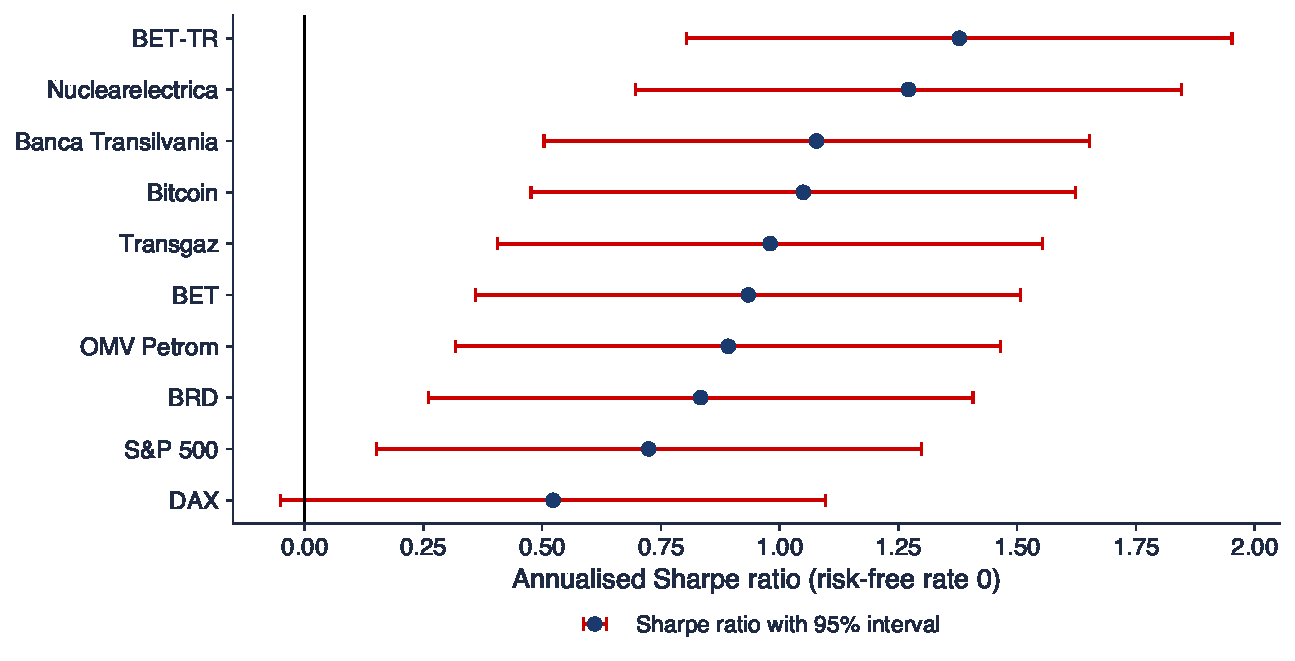
\includegraphics[width=\linewidth,height=0.80\textheight,keepaspectratio]{sfm_ch1_sharpe_ci.pdf}
\end{center}
\end{column}
\begin{column}{0.38\textwidth}
\begin{itemize}
    \item Cea mai mare estimare punctuală: BET-TR
    \item Toate intervalele se suprapun: clasamentul nu este semnificativ statistic
    \item Intervalul DAX conține 0
    \item Lățimile intervalelor sînt aproape egale: depind mai ales de lungimea eșantionului
\end{itemize}
\end{column}
\end{columns}
\quantlet{SFM\_ch1\_performance}{\qlurl{SFM_ch1_performance}}
\end{frame}

\begin{frame}{Sortino ratio}
\itemsize{\small}
\begin{itemize}
    \item Investitorii nu agreează pierderile, nu cîștigurile: volatilitatea le tratează la fel
    \item \textbf{Abaterea negativă} (downside deviation) sub un prag $\tau$ (aici $\tau = 0$)
    \begin{itemize}
        \item $\sigma_D = \sqrt{\frac1n \sum_t \min(R_t - \tau, 0)^2}$, contează doar zilele sub prag
    \end{itemize}
    \item \textbf{Sortino ratio} \refSortino: $\text{Sortino} = \dfrac{\mu - \tau}{\sigma_D}$, anualizat ca Sharpe ratio
    \item Pentru o distribuție simetrică $\sigma_D \approx \sigma/\sqrt2$, deci Sortino $\approx 1{,}4 \times$ Sharpe
    \item S\&P 500, 2015--2026: Sharpe $0{,}72$, Sortino $1{,}02$
\end{itemize}
\end{frame}

\begin{frame}{Drawdown și maximum drawdown}
\itemsize{\small}
\begin{itemize}
    \item \textbf{Drawdown}: căderea de la cel mai mare preț atins pînă acum
    \begin{itemize}
        \item $\text{DD}_t = \dfrac{P_t}{\max_{s \le t} P_s} - 1 \le 0$; zero la un nou maxim
    \end{itemize}
    \item \textbf{MDD} (maximum drawdown): $\text{MDD} = \min_t \text{DD}_t$, cea mai mare cădere de la vîrf la minim
    \begin{itemize}
        \item raportați și datele: vîrful, minimul și \textbf{recuperarea} (revenirea la vechiul vîrf)
    \end{itemize}
    \item O pierdere $x$ cere un cîștig $x/(1 - x)$ pentru recuperare
    \begin{itemize}
        \item 10\% cere 11\%; 20\% cere 25\%; 50\% cere 100\%; 80\% cere 400\%
    \end{itemize}
    \item MDD depinde de traiectorie și crește cu lungimea eșantionului \refMagdon
\end{itemize}
\end{frame}

\begin{frame}{Drawdown-uri pe întreaga istorie}
\itemsize{\footnotesize}
\begin{center}
    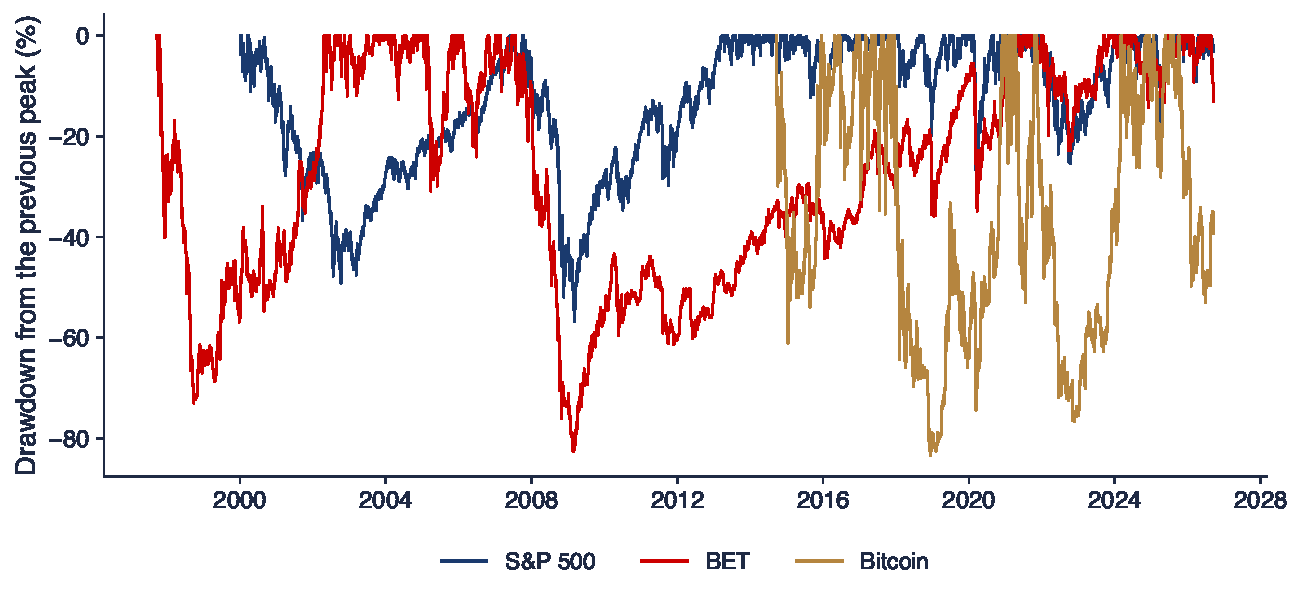
\includegraphics[width=0.97\textwidth,height=0.55\textheight,keepaspectratio]{sfm_ch1_drawdowns.pdf}
\end{center}
\vspace{-0.25cm}
\begin{itemize}
    \item S\&P 500: MDD $-56{,}8\%$, de la 9 oct. 2007 la 9 mar. 2009, recuperat pe 28 mar. 2013
    \item BET (din 1997): MDD $-82{,}5\%$, de la 24 iul. 2007 la 25 feb. 2009, recuperat abia pe 16 mar. 2021
    \item Bitcoin: MDD $-83{,}4\%$, de la 16 dec. 2017 la 15 dec. 2018
\end{itemize}
\quantlet{SFM\_ch1\_performance}{\qlurl{SFM_ch1_performance}}
\end{frame}

\begin{frame}{Cum citim graficul drawdown-urilor}
\itemsize{\small}
\begin{itemize}
    \item Adîncimea
    \begin{itemize}
        \item după un drawdown de $-82{,}5\%$, BET a avut nevoie de $+473\%$ pentru recuperare; Bitcoin, de $+502\%$
    \end{itemize}
    \item Durata
    \begin{itemize}
        \item BET a avut nevoie de 13{,}6 ani ca să revină la vîrful din 2007
        \item ponderea zilelor cu peste 20\% sub vîrf: S\&P 500 27\%, BET 56\%, Bitcoin 66\%
    \end{itemize}
    \item Volatilitatea și Sharpe ratio ignoră ordinea randamentelor; drawdown-ul nu o ignoră
    \item În perioada de comparație 2015--2026, MDD al fiecărui indice bursier a avut loc în februarie--martie 2020; Bitcoin și mai multe acțiuni BVB l-au avut la alte date
\end{itemize}
\end{frame}

\begin{frame}{Calmar ratio}
\itemsize{\small}
\begin{itemize}
    \item \textbf{Calmar ratio}: creșterea pe unitatea celei mai mari căderi, $\text{Calmar} = \dfrac{\text{CAGR}}{|\text{MDD}|}$
    \item Popular printre administratorii de fonduri: MDD este pierderea pe care investitorul chiar o trăiește
    \item S\&P 500, 2015--2026: CAGR 11{,}9\%, MDD $-33{,}9\%$
    \begin{itemize}
        \item Calmar $= 11{,}9/33{,}9 = 0{,}35$
    \end{itemize}
    \item Un singur eveniment decide numitorul: Calmar ratio este și mai zgomotos decît Sharpe ratio
    \item Comparați Calmar ratio doar pe aceeași perioadă
\end{itemize}
\end{frame}

\begin{frame}{Volatility drag}
\itemsize{\small}
\begin{itemize}
    \item Pentru un randament logaritmic cu media $m$ și varianța $\sigma^2$, randamentul simplu are media $\approx m + \sigma^2/2$
    \begin{itemize}
        \item deci rata de creștere este $\mu_{\text{log}} \approx \mu_{\text{arith}} - \sigma^2/2$
        \item diferența $\sigma^2/2$ este \textbf{volatility drag} \refBoothFama; provine din concavitatea lui $\ln$ (inegalitatea lui Jensen)
    \end{itemize}
    \item Două active cu aceeași medie aritmetică, 10\% pe an
    \begin{itemize}
        \item $\sigma = 5\%$: drag 0{,}12\%, creștere 9{,}88\% pe an; după 10 ani 1 leu devine 2{,}68
        \item $\sigma = 30\%$: drag 4{,}50\%, creștere 5{,}50\% pe an; după 10 ani 1 leu devine 1{,}73
    \end{itemize}
    \item Dublarea volatilității înmulțește drag-ul cu patru
\end{itemize}
\end{frame}

\begin{frame}{Volatility drag pe date reale}
\itemsize{\footnotesize}
\begin{columns}[T]
\begin{column}{0.56\textwidth}
\begin{center}
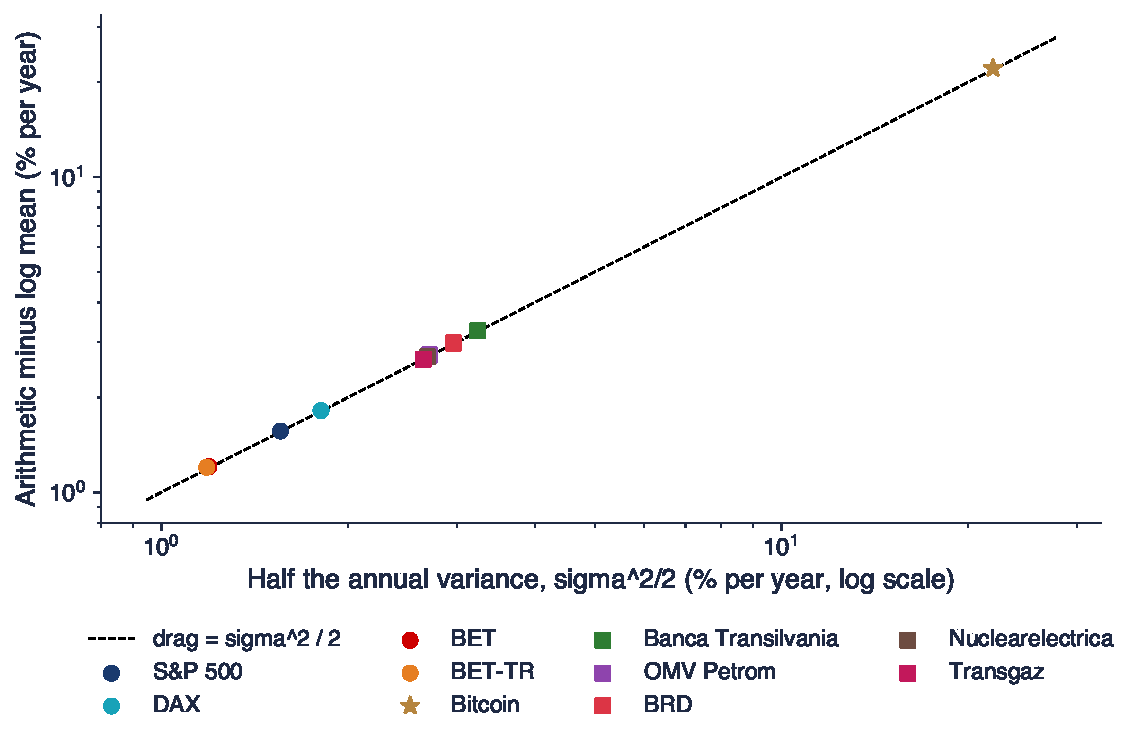
\includegraphics[width=\linewidth,height=0.80\textheight,keepaspectratio]{sfm_ch1_vol_drag.pdf}
\end{center}
\end{column}
\begin{column}{0.40\textwidth}
\begin{itemize}
    \item Fiecare punct: un activ, 2015--2026
    \item Vertical: media anuală aritmetică minus cea logaritmică; orizontal: $\sigma^2/2$
    \item Toate punctele sînt pe dreaptă: formula funcționează pe date reale
    \item Bitcoin: media aritmetică 69{,}5\%, media logaritmică 47{,}4\%, drag 22{,}1 puncte procentuale; $\sigma^2/2 = 21{,}9\%$
\end{itemize}
\end{column}
\end{columns}
\quantlet{SFM\_ch1\_volatility\_drag}{\qlurl{SFM_ch1_volatility_drag}}
\end{frame}

\begin{frame}{Întrebare pentru sală: ce randament pentru Bitcoin?}
\itemsize{\small}
\begin{itemize}
    \item Bitcoin, 2015--2026: media aritmetică a randamentelor simple 69{,}5\% pe an; CAGR 60{,}6\%
    \item \textbf{Ce credeți?} Care cifră descrie creșterea averii unui investitor?
    \item \textbf{Răspuns}
    \begin{itemize}
        \item CAGR: este rata care chiar a transformat primul preț în ultimul
        \item media aritmetică este randamentul așteptat al unui singur an, nu creșterea pe mulți ani
        \item diferența este volatility drag; pentru active cu volatilitate mică este mică
    \end{itemize}
\end{itemize}
\end{frame}

\begin{frame}{Indicatori de performanță: indici și Bitcoin, 2015--2026}
\itemsize{\small}
\begin{center}
\footnotesize
\begin{tabular}{lrrrrrrr}
\toprule
& CAGR \% & Vol. \% & Sharpe & Sortino & MDD \% & Calmar & Drag \% \\
\midrule
S\&P 500 & $11{,}9$ & $17{,}6$ & $0{,}72$ & $1{,}02$ & $-33{,}9$ & $0{,}35$ & $1{,}56$ \\
DAX & $8{,}5$ & $19{,}0$ & $0{,}52$ & $0{,}73$ & $-38{,}8$ & $0{,}22$ & $1{,}82$ \\
BET & $14{,}1$ & $15{,}4$ & $0{,}93$ & $1{,}28$ & $-31{,}1$ & $0{,}45$ & $1{,}21$ \\
BET-TR & $22{,}1$ & $15{,}4$ & $1{,}38$ & $1{,}92$ & $-31{,}1$ & $0{,}71$ & $1{,}20$ \\
Bitcoin & $60{,}6$ & $66{,}2$ & $1{,}05$ & $1{,}55$ & $-83{,}4$ & $0{,}73$ & $22{,}13$ \\
\bottomrule
\end{tabular}
\end{center}
\begin{itemize}
    \item Anualizate cu frecvența reală a fiecărei serii; Sharpe și Sortino cu $r_f = 0$
    \item Bitcoin: de departe cel mai mare CAGR, cea mai mare volatilitate și cel mai adînc drawdown
    \item BET-TR vs BET: același risc, dividendele ridică toți indicatorii bazați pe randament
\end{itemize}\quantlet{SFM\_ch1\_performance}{\qlurl{SFM_ch1_performance}}
\end{frame}

\begin{frame}{Indicatori de performanță: acțiuni BVB, 2015--2026}
\itemsize{\small}
\begin{center}
\footnotesize
\begin{tabular}{lrrrrrrr}
\toprule
& CAGR \% & Vol. \% & Sharpe & Sortino & MDD \% & Calmar & Drag \% \\
\midrule
Banca Transilvania (TLV) & $27{,}3$ & $25{,}5$ & $1{,}08$ & $1{,}59$ & $-38{,}9$ & $0{,}70$ & $3{,}25$ \\
OMV Petrom (SNP) & $19{,}7$ & $23{,}3$ & $0{,}89$ & $1{,}29$ & $-45{,}4$ & $0{,}43$ & $2{,}73$ \\
BRD & $18{,}9$ & $24{,}3$ & $0{,}83$ & $1{,}21$ & $-35{,}6$ & $0{,}53$ & $2{,}98$ \\
Nuclearelectrica (SNN) & $30{,}7$ & $23{,}2$ & $1{,}27$ & $2{,}00$ & $-36{,}8$ & $0{,}83$ & $2{,}69$ \\
Transgaz (TGN) & $22{,}0$ & $23{,}0$ & $0{,}98$ & $1{,}49$ & $-44{,}8$ & $0{,}49$ & $2{,}65$ \\
\bottomrule
\end{tabular}
\end{center}
\begin{itemize}
    \item Prețuri ajustate: dividendele sînt incluse
    \item Acțiunile individuale: volatilitate mai mare și drawdown-uri mai adînci decît indicele BET
    \item Țineți minte eroarea standard, circa $0{,}29$ pentru fiecare Sharpe ratio: diferențele mici nu sînt semnificative
\end{itemize}\quantlet{SFM\_ch1\_performance}{\qlurl{SFM_ch1_performance}}
\end{frame}

\begin{frame}{Risc și randament, 2015--2026}
\itemsize{\footnotesize}
\begin{columns}[T]
\begin{column}{0.56\textwidth}
\begin{center}
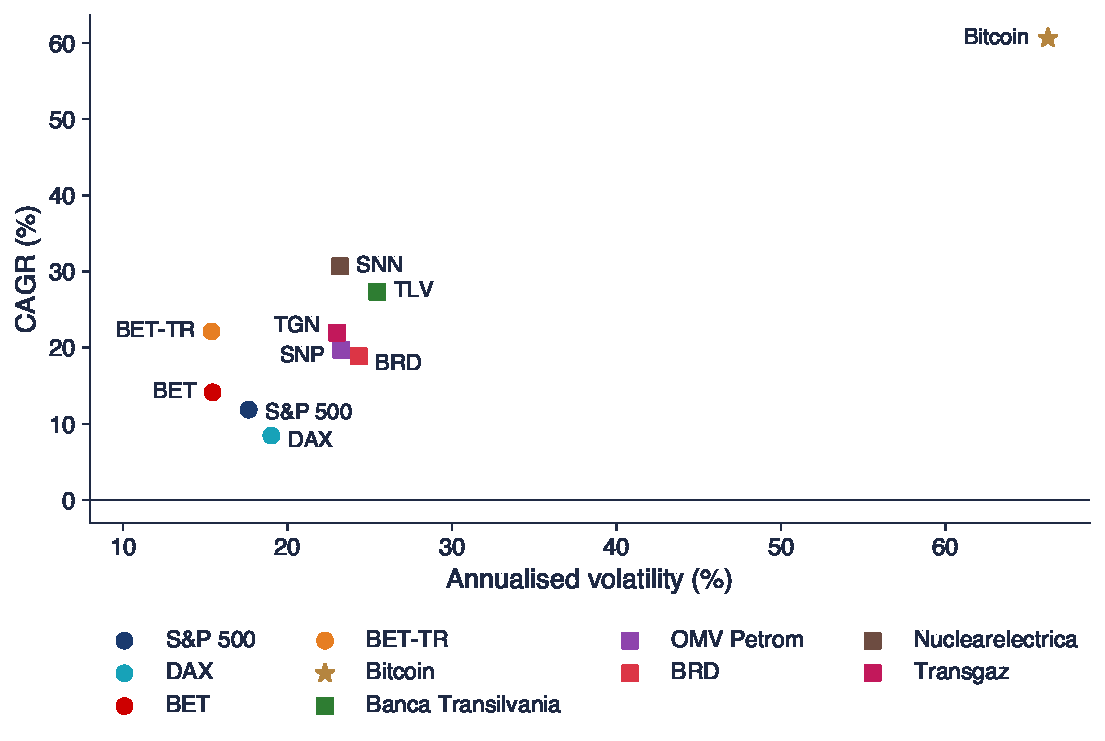
\includegraphics[width=\linewidth,height=0.80\textheight,keepaspectratio]{sfm_ch1_risk_return.pdf}
\end{center}
\end{column}
\begin{column}{0.40\textwidth}
\begin{itemize}
    \item Orizontal: volatilitatea anualizată; vertical: CAGR
    \item Cel mai bun după CAGR: Bitcoin; după Sharpe: BET-TR; după Sortino: SNN; după Calmar: SNN
    \item Cea mai mică volatilitate: BET-TR; cel mai mic MDD: BET-TR
    \item Clasamentul depinde de indicator: spuneți întotdeauna pe care îl folosiți
\end{itemize}
\end{column}
\end{columns}
\quantlet{SFM\_ch1\_performance}{\qlurl{SFM_ch1_performance}}
\end{frame}

\begin{frame}{Recapitulare: Indicatori de performanță}
\itemsize{\small}
\begin{itemize}
    \item CAGR (creștere), volatilitate (risc), Sharpe și Sortino (randament pe unitatea de risc)
    \item MDD și Calmar: cea mai mare cădere, pe care investitorul chiar o trăiește
    \item Volatility drag: $\mu_{\text{log}} \approx \mu_{\text{arith}} - \sigma^2/2$, creșterea este sub media aritmetică
    \item Fiecare indicator este o estimare: comparați diferențele cu erorile lor standard
\end{itemize}
\end{frame}


%=============================================================================
\section{AI pentru descoperire științifică}
%=============================================================================

\begin{frame}{O întrebare deschisă}
\itemsize{\small}
\begin{itemize}
    \item \textbf{Persistă Sharpe ratio în timp?}
    \begin{itemize}
        \item dacă o acțiune BVB a avut un Sharpe ratio mare în 2015--2020, l-a avut și în 2021--2026?
        \item dacă nu, clasarea fondurilor sau a acțiunilor după Sharpe ratio din trecut îi folosește puțin unui investitor
    \end{itemize}
    \item De ce este deschisă: eșantioane scurte, puține acțiuni și o eroare standard de circa $0{,}4$ pentru un Sharpe ratio estimat pe jumătate din eșantionul nostru
    \item Dovezi înrudite: multe tipare de randament publicate nu rezistă pe date noi \refHLZ
    \item Instrumentele AI pot accelera un astfel de studiu; nu înlocuiesc verificarea lui \refWang
\end{itemize}
\end{frame}

\begin{frame}{Cum ar putea ajuta AI}
\itemsize{\small}
\begin{itemize}
    \item \textbf{Literatura}: lista lucrărilor despre persistența performanței și rezumarea metodelor lor
    \item \textbf{Cod}: o primă versiune a unei funcții Python pentru Sharpe ratio pe ferestre mobile, pe datele cursului
    \item \textbf{Robustețe}: propunerea altor ferestre, altor indicatori (Sortino, Calmar), altor piețe
    \item \textbf{Explicație}: transformarea unui tabel de rezultate într-o primă versiune a interpretării
    \item Exemplu de prompt
    \begin{itemize}
        \item \aiprompt{Write a Python function that computes the annualised Sharpe ratio of daily simple returns on non-overlapping 3-year windows, with the Lo (2002) standard error.}
    \end{itemize}
\end{itemize}
\end{frame}

\begin{frame}{Ce trebuie verificat}
\itemsize{\small}
\begin{itemize}
    \item Datele: preț ajustat pentru acțiuni? același calendar pentru toate activele? perioada corectă?
    \item Formulele: factorul de anualizare ($\sqrt{252}$ vs $\sqrt{365}$), randamente simple vs logaritmice, $n$ vs $n - 1$
    \item Cifrele: recalculați două sau trei valori pe exemple mici sau cu o a doua metodă
    \item Referințele: fiecare lucrare citată trebuie să existe; verificați DOI-ul
    \item Selecția: dacă ați încercat zece ferestre, spuneți; un backtest încercat de multe ori supra-ajustează \refBBLZ
\end{itemize}
\end{frame}

\begin{frame}{Sămînță de proiect}
\itemsize{\small}
\begin{itemize}
    \item \textbf{Întrebarea}: persistă Sharpe ratio al acțiunilor BVB de la o perioadă la alta?
    \begin{itemize}
        \item date: prețurile ajustate a 10--15 acțiuni BVB, 2010--2026, din datele cursului
    \end{itemize}
    \item Pași
    \begin{itemize}
        \item împărțiți eșantionul în două jumătăți; calculați Sharpe ratio și erorile lor standard în fiecare
        \item măsurați persistența cu corelația rangurilor dintre cele două jumătăți
        \item repetați cu Sortino ratio și Calmar ratio
    \end{itemize}
    \item Rezultat: un tabel, un grafic și un paragraf despre ce pot și ce nu pot arăta datele
    \item Declarați orice folosire a AI și listați erorile AI pe care le-ați corectat
\end{itemize}
\end{frame}


%=============================================================================
\section{Rezumat}
%=============================================================================

\begin{frame}{Idei principale}
\itemsize{\small}
\begin{itemize}
    \item Verificați întîi datele: sursa, prețurile ajustate, calendarul, salturile
    \item Randamentele logaritmice se adună în timp; cele simple se adună între active
    \item Anualizați cu frecvența reală: media $\times\,q$, volatilitatea $\times\sqrt{q}$
    \item Randamentele au cozi groase, asimetrie negativă și volatilitate variabilă
    \item Judecați performanța cu mai mulți indicatori: CAGR, volatilitate, Sharpe, Sortino, MDD, Calmar
    \item Volatilitatea costă creștere: $\sigma^2/2$ pe an
    \item Randamentele medii și Sharpe ratio sînt imprecise: raportați erorile standard
\end{itemize}
\end{frame}

\begin{frame}{Formule de reținut}
\itemsize{\small}
\begin{center}
\footnotesize
\begin{tabular}{ll}
\toprule
\textbf{Mărimea} & \textbf{Formula} \\
\midrule
Randament simplu & $R_t = P_t/P_{t-1} - 1$ \\
Randament logaritmic & $r_t = \ln(P_t/P_{t-1}) = \ln(1 + R_t)$ \\
Randamente pe $k$ perioade & $1 + R_t(k) = \prod_{j=0}^{k-1}(1 + R_{t-j})$, \quad $r_t(k) = \sum_{j=0}^{k-1} r_{t-j}$ \\
Portofoliu & $R_p = \sum_i w_i R_i$ \\
Anualizare & $\mu_{\text{an}} = q\,\mu$, \quad $\sigma_{\text{an}} = \sqrt{q}\,\sigma$ \\
CAGR & $(P_T/P_0)^{1/Y} - 1$ \\
Sharpe, Sortino & $(\mu - r_f)/\sigma$, \quad $(\mu - \tau)/\sigma_D$ \\
MDD, Calmar & $\min_t \big(P_t / \max_{s \le t} P_s - 1\big)$, \quad $\text{CAGR}/|\text{MDD}|$ \\
Volatility drag & $\mu_{\text{log}} \approx \mu_{\text{arith}} - \sigma^2/2$ \\
SE a mediei, a Sharpe & $\sigma_{\text{an}}/\sqrt{Y}$, \quad $\sqrt{(1 + \text{SR}^2/2)/n}$ \\
\bottomrule
\end{tabular}
\end{center}
\end{frame}

\begin{frame}{Verificați-vă}
\itemsize{\small}
\begin{itemize}
    \item \textbf{Întrebare}: un fond raportează randamente logaritmice zilnice cu media 0,05\% și abaterea standard 1\%; care sînt media și volatilitatea anuală?
    \begin{itemize}
        \item \textbf{Răspuns}: $252 \times 0{,}05\% = 12{,}6\%$ și $\sqrt{252} \times 1\% = 15{,}9\%$
    \end{itemize}
    \item \textbf{Întrebare}: de ce este media aritmetică a randamentelor Bitcoin mult peste CAGR?
    \begin{itemize}
        \item \textbf{Răspuns}: volatility drag $\sigma^2/2$ este mare cînd $\sigma$ este mare
    \end{itemize}
    \item \textbf{Întrebare}: un indice scade cu 60\%; ce cîștig îi trebuie ca să-și revină?
    \begin{itemize}
        \item \textbf{Răspuns}: $0{,}6/0{,}4 = 150\%$
    \end{itemize}
    \item Urmează: \sfmchlink{https://danpele.github.io/SFM/RO/Cursuri/capitol2_distributii_clasice_fapte_stilizate.pdf}{Capitolul 2}, distribuții clasice și fapte stilizate ale randamentelor
\end{itemize}
\end{frame}


%=============================================================================
\section{Bibliografie}
%=============================================================================

\begin{frame}{Bibliografie (1/2)}
\itemsize{\tiny}
\begin{itemize}
    \item Bailey, D.H., Borwein, J.M., López de Prado, M., Zhu, Q.J. (2014). \href{https://doi.org/10.1090/noti1105}{Pseudo-mathematics and financial charlatanism: the effects of backtest overfitting on out-of-sample performance}. \textit{Notices of the American Mathematical Society}, 61(5), 458--471.
    \item Bailey, D.H., López de Prado, M. (2014). \href{https://doi.org/10.3905/jpm.2014.40.5.094}{The deflated Sharpe ratio: correcting for selection bias, backtest overfitting, and non-normality}. \textit{Journal of Portfolio Management}, 40(5), 94--107.
    \item Booth, D.G., Fama, E.F. (1992). \href{https://doi.org/10.2469/faj.v48.n3.26}{Diversification returns and asset contributions}. \textit{Financial Analysts Journal}, 48(3), 26--32.
    \item Borak, S., Härdle, W.K., López-Cabrera, B. (2013). \href{https://doi.org/10.1007/978-3-642-33929-5}{\textit{Statistics of Financial Markets: Exercises and Solutions}}, 2nd ed. Springer.
    \item Brown, S.J., Goetzmann, W., Ibbotson, R.G., Ross, S.A. (1992). \href{https://doi.org/10.1093/rfs/5.4.553}{Survivorship bias in performance studies}. \textit{Review of Financial Studies}, 5(4), 553--580.
    \item Campbell, J.Y., Lo, A.W., MacKinlay, A.C. (1997). \href{https://doi.org/10.1515/9781400830213}{\textit{The Econometrics of Financial Markets}}. Princeton University Press.
    \item Cont, R. (2001). \href{https://doi.org/10.1080/713665670}{Empirical properties of asset returns: stylized facts and statistical issues}. \textit{Quantitative Finance}, 1(2), 223--236.
    \item Dickey, D.A., Fuller, W.A. (1979). \href{https://doi.org/10.1080/01621459.1979.10482531}{Distribution of the estimators for autoregressive time series with a unit root}. \textit{Journal of the American Statistical Association}, 74(366), 427--431.
    \item Franke, J., Härdle, W.K., Hafner, C.M. (2019). \href{https://doi.org/10.1007/978-3-030-13751-9}{\textit{Statistics of Financial Markets: An Introduction}}, 5th ed. Springer.
    \item Harvey, C.R., Liu, Y., Zhu, H. (2016). \href{https://doi.org/10.1093/rfs/hhv059}{\ldots and the cross-section of expected returns}. \textit{Review of Financial Studies}, 29(1), 5--68.
    \item Lo, A.W. (2002). \href{https://doi.org/10.2469/faj.v58.n4.2453}{The statistics of Sharpe ratios}. \textit{Financial Analysts Journal}, 58(4), 36--52.
    \item Magdon-Ismail, M., Atiya, A.F., Pratap, A., Abu-Mostafa, Y.S. (2004). \href{https://doi.org/10.1239/jap/1077134674}{On the maximum drawdown of a Brownian motion}. \textit{Journal of Applied Probability}, 41(1), 147--161.
    \item Pele, D.T., Mazurencu-Marinescu, M. (2012). \href{https://doi.org/10.1016/j.sbspro.2012.09.1030}{Modelling stock market crashes: the case of Bucharest Stock Exchange}. \textit{Procedia -- Social and Behavioral Sciences}, 58, 533--542.
    \item Sharpe, W.F. (1966). \href{https://doi.org/10.1086/294846}{Mutual fund performance}. \textit{Journal of Business}, 39(S1), 119--138.
    \item Sharpe, W.F. (1994). \href{https://doi.org/10.3905/jpm.1994.409501}{The Sharpe ratio}. \textit{Journal of Portfolio Management}, 21(1), 49--58.
    \item Sortino, F.A., van der Meer, R. (1991). \href{https://doi.org/10.3905/jpm.1991.409343}{Downside risk}. \textit{Journal of Portfolio Management}, 17(4), 27--31.
\end{itemize}
\end{frame}

\begin{frame}{Bibliografie (2/2)}
\itemsize{\tiny}
\begin{itemize}
    \item Tsay, R.S. (2010). \href{https://doi.org/10.1002/9780470644560}{\textit{Analysis of Financial Time Series}}, 3rd ed. Wiley.
    \item Wang, H., Fu, T., Du, Y., Gao, W., et al. (2023). \href{https://doi.org/10.1038/s41586-023-06221-2}{Scientific discovery in the age of artificial intelligence}. \textit{Nature}, 620, 47--60.
\end{itemize}
\end{frame}

\end{document}
